\documentclass{ctexbook}

\usepackage{geometry}
\usepackage{placeins}
\usepackage{microtype}
\usepackage{graphicx}
\usepackage{subfigure}
\usepackage{booktabs} 
\usepackage{hyperref}
\usepackage{algorithm}
\usepackage{algorithmic}
\usepackage{amsmath}
\usepackage{amssymb}
\usepackage{mathtools}
\usepackage{amsthm}
\usepackage[textsize=tiny]{todonotes}
\usepackage{xparse}
\usepackage{physics}
\usepackage{soul}
\usepackage[skins]{tcolorbox}
\usepackage{hyperref}
\usepackage{xcolor}
\usepackage{fancyhdr}
\usepackage{minted}
\usepackage{booktabs}


% margin of the page
\fancypagestyle{main}{
    \fancyhf{}
    \renewcommand\headrulewidth{1pt}  % 页眉横线
    \renewcommand\footrulewidth{0pt}  % 页脚横线
    
    \fancyhead[OR]{\fzkai{\leftmark}}  % 页眉章标题
    \fancyhead[EL]{\fzkai{\rightmark}}  % 页眉节标题
    \fancyfoot[OC,EC]{\thepage}  % 页码
}
\pagestyle{main}
\geometry{
  a4paper,
  left=3cm,
  right=3cm,
  top=2.54cm,
  bottom=2.54cm,
  headheight=1.5cm,
  headsep=10pt
}


% links
\hypersetup{
    CJKbookmarks=true,
    colorlinks=true,
    breaklinks=true,
}


% graphics
\graphicspath{ {assets/figures/} }
\DeclareGraphicsExtensions{.png, .pdf}


% theorems
\theoremstyle{plain}
\newtheorem{theorem}{Theorem}[section]
\newtheorem{proposition}[theorem]{Proposition}
\newtheorem{lemma}[theorem]{Lemma}
\newtheorem{corollary}[theorem]{Corollary}
\theoremstyle{definition}
\newtheorem{definition}[theorem]{Definition}
\newtheorem{assumption}[theorem]{Assumption}
\theoremstyle{remark}
\newtheorem{remark}[theorem]{Remark}


% colors
\definecolor{g1}{HTML}{7be495}
\definecolor{b1}{HTML}{1eb0bb}


% chatting box
\tcbuselibrary{breakable, listings} %breakable:支持跨页
\newtcolorbox[
    auto counter, 
    number within=section, 
    list type=section, 
    list inside=toc]{promptbox}[1]{
        colback=white, 
        colframe=g1, %背景和线条颜色
        colbacktitle=g1, 
        coltitle=white, %标题框的背景和线条颜色 
        fonttitle=\bfseries, 
        title={读者提问 \thetcbcounter}, 
        list entry={读者提问 \thetcbcounter\quad}, %标题
        breakable, %支持跨页
        before upper={\parindent10pt\noindent},  % 支持缩进。\noindent:首行不缩进
        left = 1 mm, %文字离线框左边的边距
        right = 1 mm, %同上
        top = 1 mm, %同上
        bottom = 1 mm,%同上
        left skip = 0.25\textwidth,
        % arc is angular = 1mm, % 棱角线框
        % sharp corners, % 直角线框
        % enhanced,frame hidden, % 隐藏线框
        enhanced,drop fuzzy shadow,  % 显示阴影
}

\newtcolorbox[
    auto counter, 
    number within=section, 
    list type=section, 
    list inside=toc]{gptbox}[1]{
        colback=white, 
        colframe=b1, %背景和线条颜色
        colbacktitle=b1, 
        coltitle=white, %标题框的背景和线条颜色 
        fonttitle=\bfseries, 
        title={AI作答 \thetcbcounter}, 
        list entry={AI作答 \thetcbcounter\quad}, %标题
        breakable, %支持跨页
        before upper={\parindent10pt\noindent},  % 支持缩进。\noindent:首行不缩进
        left = 1 mm, %文字离线框左边的边距
        right = 1 mm, %同上
        top = 1 mm, %同上
        bottom = 1 mm,%同上
        right skip = 0.10\textwidth,
        % arc is angular = 1mm, % 棱角线框
        % sharp corners, % 直角线框
        % enhanced,frame hidden, % 隐藏线框
        enhanced,drop fuzzy shadow,  % 显示阴影
}

\lstset{
    basicstyle=\ttfamily\small,  % 字体和大小
    commentstyle=\color{gray},  % 注释颜色
    keywordstyle=\color{blue},  % 关键字颜色
    stringstyle=\color{red},    % 字符串颜色
    breaklines=true,            % 自动换行
    numbers=left,               % 行号在左侧显示
    numbersep=-10pt,
    showspaces=false,           % 不显示空格
    columns=fixed,              % 字间距固定
    % frame=shadowbox,            % 添加阴影边框
    % rulesepcolor=\color{gray}   % 边框颜色
}


% common commands
\NewDocumentCommand \fig       { D[]{ht} m }{  
    \begin{figure}[#1]                     
        \centering          
        {#2}
    \end{figure}                       
}                  
\NewDocumentCommand \widefig   { D[]{ht} m m m }{
    \begin{figure*}[#1]
        \centering
        {#3}
        \caption{#2}
        {#4}
    \end{figure*}
}
\NewDocumentCommand \tab       { D[]{ht} m m }{ 
    \begin{table}[#1]
        \caption{#2}
        \centering
        {#3}
    \end{table}    
}                    
\NewDocumentCommand \widetab   { D[]{ht} m m }{
    \begin{table*}[#1]
        \caption{#2} 
        \centering
        {#2}
    \end{table*}
}
\NewDocumentCommand \alg       { D[]{ht} m m }{
    \SetAlgoCaptionLayout{capleft}
    \setlength{\algomargin}{1.2em}  % left space of algo contents
    \SetAlgoCaptionSeparator{ }
    \begin{algorithm}[{#1}]
        \DontPrintSemicolon
        \SetKwInOut{Input}{\bfseries Input}  % \Input{xxx}
        \SetKwInOut{Output}{\bfseries Output}  % \Output{xxx}
        \caption{{#2}}
        {#3}  % \ForEach{xxx}{ xxx\; \If{xxx}{ xxx\; } }
    \end{algorithm}
}
\NewDocumentCommand \equ       { m }{
    \begin{equation}
        {#1}
    \end{equation}
}
\NewDocumentCommand \lst       { m }{
    \begin{itemize}
        {#1}
    \end{itemize}
}
\NewDocumentCommand \enu       { m }{
    \begin{enumerate}
        {#1}
    \end{enumerate}
}

\NewDocumentCommand \refalg    { m }{Algorithm~\ref{#1}}
\NewDocumentCommand \refequ    { m }{Equation~\ref{#1}}
\NewDocumentCommand \reffig    { m }{Figure~\ref{#1}}
\NewDocumentCommand \reftab    { m }{Table~\ref{#1}}
\NewDocumentCommand \refsec    { m }{第\ref{#1}节}
\NewDocumentCommand \refapp    { m }{Appendix \ref{#1}}
\NewDocumentCommand \refdef    { m }{Definition \ref{#1}}
\NewDocumentCommand \refthm    { m }{Theorem \ref{#1}}
\NewDocumentCommand \refpro    { m }{Proposition \ref{#1}}
\NewDocumentCommand \reflem    { m }{Lemma \ref{#1}}
\NewDocumentCommand \refrem    { m }{Remark \ref{#1}}

\NewDocumentCommand \hlt       { D[]{blue} m }{\sethlcolor{#1} \hl{#2}}


% User-defined commands
\newcommand{\prompt}[1]{
\begin{promptbox}
s \footnotesize{#1}
\end{promptbox}
}
\newcommand{\gpt}[1]{
\begin{gptbox}
s \footnotesize{#1}
\end{gptbox}
}

\NewDocumentCommand \gptc { D[]{cyan} m }{ \textcolor{#1}{#2} }

% 定义带变量的命令
\NewDocumentCommand \customPrompt { m m }{%
    \begin{tcolorbox}[boxrule = 0pt,arc = 0pt,left = 0pt,right = 0pt,top = 0pt,bottom = 0pt,colback = #1!20]
        \sethlcolor{#1}\hl{#2}
    \end{tcolorbox}%
}



\begin{document}

\chapter{A}
\chapter{B}

\chapter{AIGC: 点亮内容创作的未来}
% \section{介绍}\label{sec:intro}

\prompt{什么是AIGC技术?}


\gpt{
AIGC(Artificial Intelligence Generated Content)即人工智能生成内容,是指通过人工智能技术自动生成各种类型的内容,包括文本、图像、音频、视频等。其核心思想是利用人工智能算法,通过已有数据的学习和识别,生成具有一定创意和质量的内容。
AIGC技术主要基于以下几种核心技术。
1)深度学习:通过神经网络等模型对大量数据进行学习,从而生成新的内容。
2)自然语言处理(NLP):用于理解和生成文本内容,是AIGC生成文本内容的基础。
3)计算机视觉:用于图像和视频的生成与处理。
4)生成对抗网络(GAN):通过生成器和判别器的对抗训练生成新的内容。
AIGC技术的应用范围非常广泛,涵盖了内容创作、数据分析、产品设计等多个领域。例如,在文学创作、广告设计、教育培训等领域,AIGC能够快速生成高质量的内容,提高创作效率。
}

以上对话就是根据用户的提问由人工智能生成的内容(AIGC),其中的核心模块是人工智能领域的GPT模型。
GPT(Generative Pre-trained Transformer)是一种基于Transformer架构的大型语言模型,主要用于自然语言处理和生成任务。它最初由OpenAI开发,如今全球许多公司和研究机构也纷纷涉足类似技术的开发,例如国内的百度、阿里巴巴、腾讯,以及国外的LinkedIn、Microsoft等。这些模型在学术、商业、教育等多个领域得到了广泛应用,包括文献搜索、论文阅读、写作辅助、智能客服、内容创作、个性化学习、语言教学等,显著提高了工作效率和质量。

本章将从实践的角度和读者一起探索AIGC的博大精深,面向信息搜索、文献阅读、写作、代码编写、AI辅助办公和设计等场景,运用GPT模型为读者自动生成解决方案。






% \section{GPT辅助搜索}\label{sec:gpt-aided-writing}

在当今信息爆炸的时代,高效的信息检索已成为学术研究和日常生活中不可或缺的一部分。GPT模型作为一种强大的语言生成工具,在辅助搜索领域展现出显著的便利性和高效性。本节将从通用搜索和文献搜索两个方面,深入探讨GPT模型在信息检索中的应用。
首先,在通用搜索方面,GPT模型通过其强大的自然语言处理能力,能够为用户提供更加精准和个性化的搜索结果。例如,Search-GPT是一款将GPT引擎直接应用于搜索结果的工具,它能够结合先进的语言处理技术,快速生成准确且相关的搜索结果。此外,GPT模型还支持多模态输入,能够处理文本、图像等多种形式的信息,进一步提升了搜索的灵活性和准确性。
在文献搜索方面,GPT模型的应用则更为广泛和深入。例如,GPT Researcher工具能够根据给定的研究问题或主题,自动生成文献综述,并从海量学术资源中提取关键信息。此外,该工具还具备智能论文摘要生成功能,能够帮助研究人员快速了解文献的核心内容,从而节省大量阅读时间。通过这种自动化的文献检索和信息提取,GPT模型极大地简化了学术研究的过程,使研究人员能够更加专注于核心研究任务。

因此,GPT模型在辅助搜索领域的应用不仅提升了信息检索的效率,还为学术研究和日常信息获取提供了强大的支持。无论是通用搜索中的多模态信息处理,还是文献搜索中的自动化文献综述和摘要生成,GPT模型都展现出巨大的潜力和价值。

\subsection{通用信息检索}

对于广大用户而言,GPT不仅仅是一个简单的语言模型,更像是一位多功能的智囊团,能够为生活的各个方面提供精准且高效的建议和解决方案。
GPT模型通过其强大的自然语言处理能力,能够理解并生成高质量的文本内容,从而在学习、工作和生活等多个领域发挥重要作用。例如,在旅行规划方面,用户无需自行收集和整理复杂的天气、地理和人文信息,而是可以直接向GPT提出具体问题。模型能够基于其预训练的海量数据和强大的推理能力,快速生成综合性的建议。这些建议不仅涵盖了目的地的气候条件、地理环境和文化特色,还可能包括交通路线规划、住宿推荐以及当地风俗习惯等内容,从而为用户提供全面且个性化的出行方案。
这种能力的实现,得益于GPT模型的多模态输入和输出特性,以及其对复杂信息的高效整合能力。通过自然语言交互,用户可以轻松获取所需信息,而无需耗费大量时间和精力进行繁琐的信息检索和整理。这种高效的信息获取方式,不仅极大地提升了个人的生活效率,还为用户在面对复杂决策时提供了有力支持。
此外,GPT模型的应用场景远不止于旅行规划。在学习领域,它能够为学生提供个性化的学习计划和知识解答;在工作场景中,它可以协助专业人士进行数据分析、文案撰写和项目规划;在日常生活中,它还可以为用户提供健康咨询、饮食建议和休闲活动推荐等。通过这种全方位的支持,GPT模型正在逐渐成为现代生活中不可或缺的智能助手,为人们的生活带来更多便利和可能性。

例如,当读者需要确定出行计划,可以不用自己收集天气,地理和人文的多样的因素,直接向AI提问就能得到建议:

\prompt{北京天气如何,今天下午适合去参观故宫还是长城?}
\gpt{北京今天下午 15-18 点天气均为晴,气温在 2℃-11℃。更建议去参观故宫,原因如下:

时间方面:故宫在淡季虽然 15:30 停止检票,16:30 闭馆,但如果合理规划,在一个小时内可以游览部分核心区域,比如沿着中轴线参观三大殿等重要建筑,能在闭馆前有较好的参观体验。
交通便利性方面:故宫位于市区,交通十分便利,从时间和精力的消耗上相对较少,能把更多时间用于参观游览。

相比之下,虽然长城在晴天视野开阔,景色壮观,但长城地处户外,风相对较大,体感较冷,需要做好保暖防风措施,携带厚外套、帽子、手套等。且前往长城的交通用时较长,如果选择公交或地铁转乘,到达后可用于游玩的时间会比较紧张,游玩体验可能会受影响。}

对于不明白的概念,AI也能帮助我们理解。比如,对于高中生来说,自己学量子力学相关概念困难重重,可以尝试求助AI:

\prompt{量子叠加态和量子纠缠等有什么关系?}

\gpt{第一,量子叠加态是量子纠缠的基础,正是因为量子具有叠加态这种特性,才使得量子之间能够形成纠缠这种特殊的关联状态。第二,量子纠缠是量子叠加态在多个量子系统中的一种特殊表现形式,多个量子通过纠缠形成一种相互关联的叠加态,使得对其中一个量子的测量结果会瞬间影响到另一个处于纠缠态的量子,而不论它们相隔多远。}

日常生活中,有很多场景需要收集各种复杂繁琐的信息,如设备的参数。这时AI能够快速帮读者阅读在线网页并汇总分析,给出权衡之后的建议,为读者节省大量时间:

\prompt{请给出5000价位段最受欢迎的两款笔记本电脑型号,并总结其与同价位产品的优势。}

\gpt{5000 价位段受欢迎的两款笔记本电脑及与同价位产品相比的优势如下:

    联想 ThinkBook 14+ 2024:拥有丰富接口,像 TGX 接口可外接显卡、还有 RJ45 网口等,且有独显版可选,性能释放强劲,屏幕为 3K 分辨率的高素质 IPS 屏更护眼。
    联想小新 Pro14:屏幕是 2.8k 分辨率的 OLED 屏,色彩显示极为出色,且体型相对轻薄小巧,便于携带。
}

\prompt{如果追求性能,那款更具性价比?}

\gpt{如果追求性能,联想 ThinkBook 14+ 2024 更具性价比,因为它不仅有独显版本可选,能实现更高的 GPU 渲染能力,其散热系统也更强大,可实现 70W 的 CPU 单烤,且内存和硬盘容量有更多高配置可选。}

\subsection{文献搜索引擎}

在学术研究中,快速获取最新的学术文献是进行文献回顾和信息收集的重要环节。近年来,随着人工智能技术的发展,GPT模型及其相关工具在学术文献搜索领域展现出了显著的优势。这些工具不仅能够快速定位最新的学术成果,还能通过智能总结和分析,为研究人员提供高效的文献检索体验。
例如,PaSa 是字节跳动研究团队推出的基于强化学习的学术论文检索智能体,能够模仿人类研究者的行为,自动调用搜索引擎、浏览相关论文并追踪引文网络。它通过其核心组件 Crawler 和 Selector 实现高效的信息处理,能够在两分钟内完成一次详尽的学术调研,其检索速度和准确性均优于传统的搜索引擎。此外,PaSa 还支持复杂学术查询,能够理解并处理涉及特定算法或研究方法的细粒度问题。
另一个值得关注的工具是 OpenScholar,这是一个由华盛顿大学 NLP 实验室和 Ai2 等机构合作开发的开源学术搜索工具。OpenScholar 通过检索增强的语言模型,结合一个包含 4500 万篇论文的数据库,能够快速回答用户的学术查询,并生成基于这些来源的回答。其性能在多个学科领域中均优于 GPT-4o 和其他专用文献综述系统。
此外,Inciteful 作为一个先进的学术文献搜索和分析平台,通过构建引用网络帮助研究人员发现和连接相关学术文献。它支持交互式可视化展示,能够快速定位相关文献,并提供文献之间的引用路径,从而帮助研究人员高效地掌握特定领域的研究动态。
这些基于 GPT 模型的工具和平台,通过其强大的自然语言处理能力和智能检索功能,为研究人员提供了前所未有的便利。它们不仅能够快速定位最新的学术成果,还能通过自动化的文献总结和分析,帮助研究人员在前期文献回顾阶段节省大量时间和精力,从而更专注于核心研究任务。

具体而言,GPT擅长帮助读者:
\begin{itemize}
    \item 查询最新的研究论文
    \item 总结领域研究进展
    \item 对某领域的研究进行一个简要的分析
    \item 对所提供的具化智能体相关论文进行摘要总结
\end{itemize}

例如,读者可以直接向AI提问关于某个领域的发展概况:
\prompt{去年到现在自然语言处理领域有什么重要的新发现?}
\gpt{从去年到现在,自然语言处理(NLP)领域取得了多个重要进展。最显著的可能是大规模语言模型的持续优化和多模态能力的提升。像GPT-4和ChatGPT等大规模模型在理解和生成文本方面的表现更加精准,能够更好地处理复杂的语境和任务。同时,跨模态学习开始兴起,模型不仅能处理文本,还能结合图像、音频等其他数据形式,提升了在实际应用中的灵活性和准确性。另外,增强学习与自监督学习方法的进一步发展,使得模型在少量标注数据或无标注数据下也能表现出色。最后,在AI伦理和可解释性方面,学者们加强了对算法透明度和偏见的关注,推动了更加负责任的AI研发。}

除此之外,读者能够通过提问获取满足需要的论文及其简单描述。
\prompt{查询近三年关于图神经网络可解释性的研究论文}
\gpt{
以下是近三年关于图神经网络(GNN)可解释性的研究论文:

GraphLIME: Local Interpretable Model Explanations for Graph Neural Networks
本文提出了GraphLIME,一种基于Hilbert-Schmidt独立性准则(HSIC)Lasso的非线性特征选择方法,用于解释GNN模型的局部可解释性。实验表明,GraphLIME在解释性和描述性方面优于现有方法。

How Interpretable Are Interpretable Graph Neural Networks?
本文提出了一种新的XGNN架构,称为Graph Multilinear neT (GMT),通过多线性扩展理论框架提高了子图的可解释性和泛化能力,在多个图分类基准上表现优异。

Explainability in Graph Neural Networks: A Taxonomic Survey
本文提供了GNN可解释性方法的统一分类视图,并建立了一个标准化的测试平台,以便对各种技术进行比较和分析。

Evaluating explainability for graph neural networks
本文介绍了一种合成图数据生成器S HAPE GG EN,用于生成带有真实解释的基准数据集,以评估GNN解释方法的质量和可靠性。

Learning to Explain Graph Neural Networks
本文提出了L2xGnn框架,通过选择解释性子图来提供忠实的解释,确保仅使用提供的解释进行预测,同时保持与基线方法相同的分类准确性。

}

为了能够搞清楚某个略有具体的技术和方法演进,读者可以使用特定的AI工具快速梳理该领域论文的引用关系网络,从而快速识别不用方法之间的关系和脉络。以Research Flow\footnote{\url{https://rflow.ai}}为例,所有论文之间的引用关系网络如\reffig{fig:cite-network}所示。

\prompt{Mamba: Linear-Time Sequence Modeling with Selective State Spaces}

\fig{
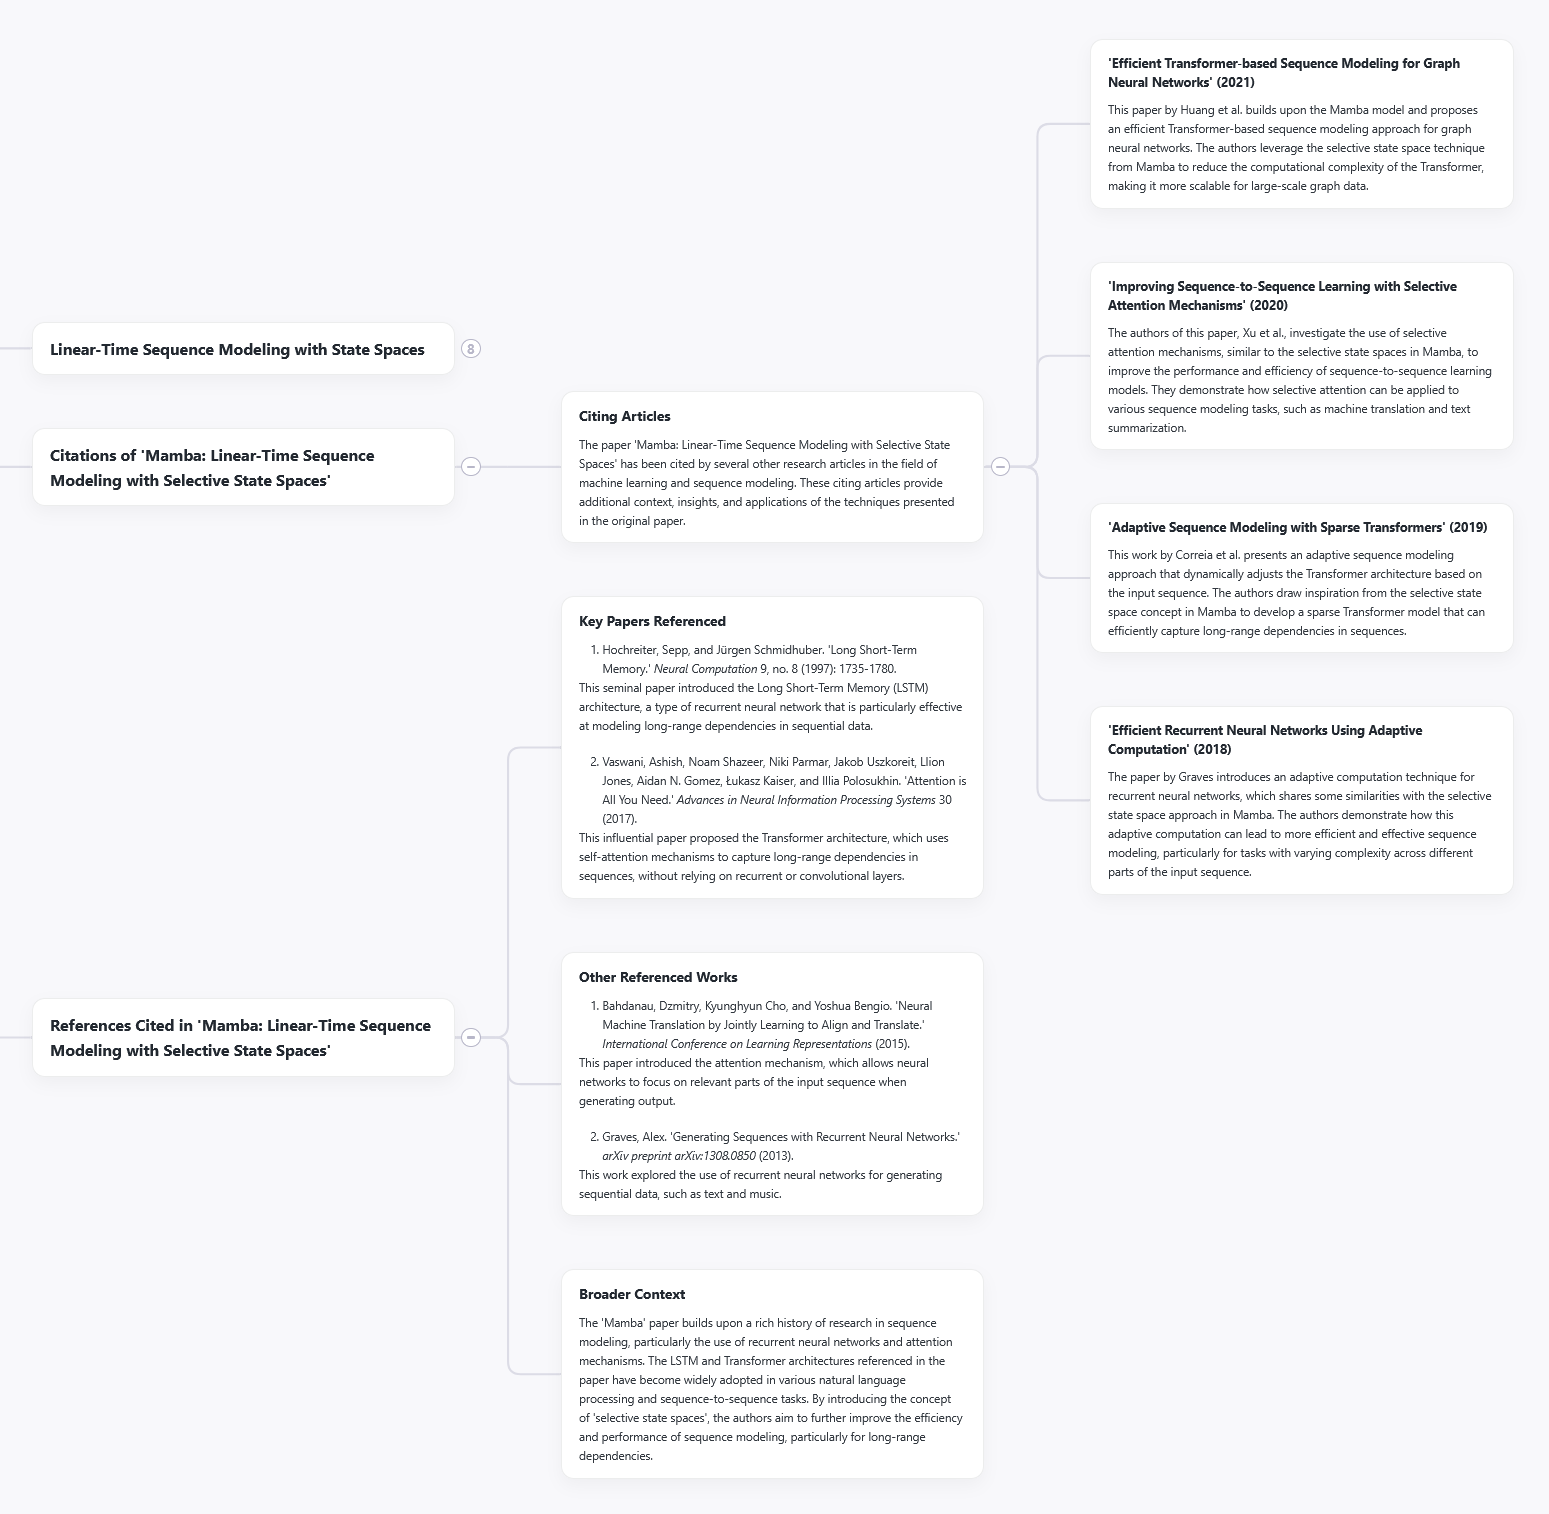
\includegraphics[width=1\textwidth]{assets/figures/cite-network}
\caption{Research Flow中的论文被引和引用关系} 
\label{fig:cite-network}
}

% \section{GPT辅助文献查找和阅读}

AI的GPT模型不仅能够帮助读者检索信息,还能够分析和整理收集到的信息,归纳为便于阅读的重点内容,帮助读者快速理解大量信息。下面由浅入深从多个方面进行解读。

\subsection{快速概括论文内容}
论文长度一般几页到几十页不等,加上复杂的表述,往往需要花费大量时间阅读额,AI能够快速处理论文中的信息,并未读者生成高度凝练的概括性文字。读者只需要将论文的标题、摘要和引言部分输入AI工具,要求其用简洁的语言总结论文的主要观点、研究方法和结论。例如:
\prompt{请用简洁的语言概括以下论文的主要观点、研究方法和结论:《基于深度学习的图像识别技术研究》。}
\gpt{本文主要研究了基于深度学习的图像识别技术,通过卷积神经网络(CNN)对大量图像数据进行训练,实现了高精度的图像分类和识别。实验结果表明,该技术在多个标准数据集上表现出色,准确率超过95\%。}

\subsection{提取关键信息}
论文中的关键信息往往对全文贡献巨大,能够体现整篇文章的贡献,因此提取关键信息也是阅读论文的重中之重。对此,读者只需要稍微调整提问方式,将论文的主要部分(如方法、结果、讨论)输入AI工具,要求其提取关键信息和要点,即可用过AI得到论文的关键信息:
\prompt{请提取以下论文的关键信息和要点:《深度学习在自然语言处理中的应用研究》。}
\gpt{关键信息:\\
     研究背景:自然语言处理(NLP)在人工智能领域的重要性。\\
     研究方法:使用Transformer架构的预训练模型(如BERT、GPT)进行文本分类、情感分析和机器翻译。\\
     实验结果:在多个NLP任务上,预训练模型的性能显著优于传统方法。\\
     结论:预训练模型在自然语言处理领域具有广泛的应用前景。\\
}

\textbf{AI fact-checking paper(AI事实核查论文解读)}。
在处理涉及事实核查的论文时,这个工具能够帮助你理解并解读相关的研究。它能解释论文的核心观点,总结关键发现,甚至批判 AI 在事实核查中的角色。
示例用法:
\begin{itemize}
    \item 你能解释一下这篇论文的主要论点吗
    \item 关于人工智能在事实核查中的关键发现是什么
    \item 这篇论文是如何批评人工智能在事实核查中的作用的
    \item 你能总结一下这项研究的结论吗
\end{itemize}

\prompt{Learning to Walk across Time for Interpretable Temporal
 Knowledge Graph Completion这篇论文是如何说明模型的可解释性的?}
\gpt{
    \item 在论文 "Learning to Walk across Time for Interpretable Temporal Knowledge Graph Completion" 中,作者提出了一种新的模型,该模型通过模拟在知识图谱上“行走”的过程来学习时间依赖关系,并强调了模型的可解释性。以下是该论文中关于模型可解释性的几个关键点:
    \item\textbf{基于路径的推理}:模型通过在知识图谱上模拟行走(即沿着实体和关系的路径移动)来推理。这种行走过程可以视为一种基于路径的推理方法,其中每一步都依赖于当前时间戳和图谱中的信息。这种基于路径的方法自然地提供了一种解释预测结果的方式,因为可以通过展示行走路径来解释模型是如何得出特定预测的。
    \item \textbf{时间敏感的行走}:模型在行走过程中考虑了时间因素,这意味着它能够理解实体之间的关系如何随时间变化。这种时间敏感的行走不仅提高了模型的预测准确性,还使得模型能够提供关于预测随时间变化的解释。
    \item \textbf{可视化解释}:为了进一步提高模型的可解释性,论文可能探讨了如何可视化模型的行走路径。通过可视化模型在知识图谱上的行走路径,研究人员和用户可以更直观地理解模型的决策过程。
    \item \textbf{对比分析}:论文可能还讨论了如何通过对比分析来增强模型的可解释性。例如,通过比较不同行走路径或不同时间点的模型预测,可以揭示模型在不同情况下的行为差异,从而提供更深入的解释。
    \item \textbf{模型评估}:在评估模型的可解释性时,论文可能考虑了模型在不同数据集和任务上的表现,以及模型预测的一致性和稳定性。这些评估有助于验证模型的可解释性是否与其预测性能相匹配。
    总的来说,该论文通过提出一种基于时间敏感行走的模型,并强调模型的可解释性,为时间知识图谱补全任务提供了一种新的解决方案。通过可视化模型的行走路径和提供基于路径的推理,该模型能够为用户提供更直观、更可信的解释。
}

\subsection{解析专业术语}
对于论文中频繁出现的专业术语,初次接触的读者难免会不解或产生误解,影响论文的阅读质量和阅读速度。AI非常擅长对特定名词进行解释,同时其还会结合论文的上下文,对特定概念进行一定的扩展和延申,让读者更容易获取论文的核心思想。
\prompt{请解释以下专业术语:卷积神经网络(CNN)。}
\gpt{卷积神经网络(Convolutional Neural Network, CNN)是一种深度学习模型,主要用于图像识别和处理。它通过卷积层、池化层和全连接层的组合,自动提取图像中的特征,具有强大的特征学习能力。}
\prompt{Mamba论文中的ssm是什么意思?简述其作用}
\gpt{在 Mamba 模型中,SSM(State Space Model,状态空间模型)是一种用于高效序列建模的核心组件,其作用是通过递归更新状态向量来处理序列数据。Mamba 对 SSM 进行了改进,引入了选择性机制(Selective State Space Model,简称 S6),使得模型能够根据输入动态调整参数,从而选择性地关注重要信息并忽略不重要的内容。
具体来说,SSM 在 Mamba 中的作用包括:
高效处理长序列:SSM 的计算复杂度仅为 O(N),适合处理长序列。
选择性信息处理:通过动态调整参数(如矩阵 B、C 和步长 Δ),模型可以根据输入的重要性选择性地保留或忽略信息。
结合硬件感知算法:优化计算效率,减少内存访问,提升模型的训练和推理速度。
此外,SSM 的选择性机制类似于 Transformer 中的注意力机制,但更适合在状态空间模型框架下实现,能够有效解决传统 SSM 参数固定带来的灵活性不足问题。}

\subsection{生成结构化笔记}
对于结构复杂的文献,如果能够根据逻辑关系快速生成要点,形成结构化的文档,将为读者提供积极的指导作用。下面给出一个例子。

\prompt{请为这篇论文生成一个基于IMRAD(引言、方法、结果、讨论)的笔记:《基于深度学习的图像识别技术研究》。}


\begin{gptbox}
\footnotesize{
引言:
    \begin{itemize}
        \item {研究背景:图像识别在计算机视觉领域的应用。}
        \item {研究目的:提高图像识别的准确性和效率。}
    \end{itemize}
    
    \begin{itemize}
        \item {数据集:使用ImageNet数据集进行训练和测试。}
        \item {模型:采用卷积神经网络(CNN)架构。}
        \item {实验设计:对比不同网络结构的性能。}
    \end{itemize}
结果:
    \begin{itemize}
        \item {准确率:在测试集上达到95\%的准确率。}
        \item {效率:训练时间比传统方法缩短了30\%。}
    \end{itemize}
讨论:
    \begin{itemize}
        \item {优势:模型具有良好的泛化能力和高准确率。}
        \item {局限性:对计算资源要求较高。}
        \item {未来工作:探索更高效的网络结构和优化算法。}
    \end{itemize}
}
\end{gptbox}

\subsection{对比分析文献}
对比式学习是最重要的学习方法之一,AI能够运用其快速数据处理能力,为用户提供不同方法和文献之间的差异和共通之处,帮助读者融汇贯通不同的知识。下面的例子通过指令让AI工具对比不同文献的研究设计、样本大小、结果和结论,并分析它们在研究方法和发现上的异同点。
\prompt{请对比以下两篇文献的研究设计、样本大小、结果和结论,并分析它们在研究方法和发现上的异同点:
    \begin{itemize}
        \item {文献1:《基于深度学习的图像识别技术研究》}
        \item {文献2:《传统机器学习在图像识别中的应用》}
    \end{itemize}
}
\gpt{研究设计:
    \begin{itemize}
        \item {文献1:使用卷积神经网络(CNN)进行图像识别。}
        \item {文献2:使用支持向量机(SVM)进行图像识别。}
    \end{itemize}
    \item {样本大小:}
    \begin{itemize}
        \item {文献1:使用ImageNet数据集,包含超过1000万张图像。}
        \item {文献2:使用自建数据集,包含10万张图像。}
    \end{itemize}
    \item {结果:}
    \begin{itemize}
        \item {文献1:准确率达到95\%。}
        \item {文献2:准确率达到85\%。}
    \end{itemize}
    \item {结论:}
    \begin{itemize}
        \item {文献1:CNN在图像识别中表现出色,适合大规模数据集。}
        \item {文献2:SVM在小规模数据集上表现良好,但对大规模数据集的泛化能力有限。}
    \end{itemize}
    \item {异同点:}
    \begin{itemize}
        \item {相同点:两者都用于图像识别任务。}
        \item {不同点:CNN在处理大规模数据集时表现更好,而SVM在小规模数据集上效率更高。}
    \end{itemize}
}

\subsection{文献管理与总结}
在学术研究的进程中,随着研究的不断深入,研究者所接触的文献数量往往会呈现出显著的增长趋势。这一现象不仅反映了研究主题的复杂性与多维度性,也对研究者的信息整理能力提出了更高的要求。当面对海量的文献资料时,如何高效地对其进行分类、整理以及深度挖掘,成为研究者必须面对的重要课题。

在这一过程中,对每一篇重要文献进行深入的总结与分析显得尤为关键。这种总结并非简单的信息罗列,而是一种深度的信息提取与整合,旨在提炼文献的核心观点、研究方法、结论以及与其他研究的关联性。借助现代科技的力量,人工智能工具(AI)在此环节中发挥了不可替代的作用。AI工具能够凭借其强大的数据分析与处理能力,快速而精准地对文献内容进行梳理,提炼出关键信息,并以简洁明了的方式呈现出来。这种高效的总结方式不仅节省了研究者大量的时间和精力,还能够帮助研究者更清晰地把握文献的脉络与重点,从而为进一步的研究提供坚实的基础。

然而,仅对文献进行总结是远远不够的。为了更好地管理和运用这些总结信息,研究者需要借助专业的文献管理工具。例如,Zotero和Mendeley等工具以其强大的功能和便捷的操作,成为众多研究者的首选。这些工具不仅能够帮助研究者对文献进行分类存储,还能够实现文献的标注、引用以及与其他文献的关联分析。通过将AI工具生成的文献总结内容保存在这些文献管理工具中,研究者可以构建起一个系统化、结构化的文献知识库。在这个知识库中,每一篇文献的总结都如同一颗颗珍珠,被有序地串联起来,形成一个完整的学术研究脉络。如此一来,研究者在后续的研究过程中,无论是进行文献回顾、理论构建还是实证分析,都能够快速地找到所需的信息,从而大大提高研究效率,提升学术研究的质量与深度。

另外,文献在的表示具有严格的规范,下面的例子给出了文献引用需要用到的参考文献,为初学者提供了学习参考。
\prompt{请为这篇论文生成一个简要总结,并提取关键引用信息:
    \begin{itemize}
        \item {文献:《基于深度学习的图像识别技术研究》}
        \item {引用格式:APA}
    \end{itemize}
}
\gpt{
    \begin{itemize}
           \item 论文简要总结
           \item 论文标题:基于深度学习的图像识别技术研究
           \item 作者:[作者姓名]
           \item 发表年份:[具体年份]
           \item 期刊名称:[期刊名称]
           \item 摘要:
            本文综述了深度学习在图像识别领域的应用,重点探讨了卷积神经网络(CNN)在图像分类、目标检测和语义分割中的表现。文章分析了CNN的架构设计与优化方法,并讨论了当前技术面临的挑战及未来研究方向,如迁移学习和多模态融合。
            \item 关键引用信息(APA格式)
            \item 文中引用:
            ([作者姓名], [具体年份])
            [作者姓名]([具体年份])探讨了CNN在图像识别中的应用。
            参考文献列表:
            [作者姓名]. ([具体年份]). 基于深度学习的图像识别技术研究. [期刊名称], [卷号], [起始页码]-[结束页码].
            \item 示例:
            文中引用:(张三, 2023)
            张三(2023)探讨了CNN在图像识别中的应用。
            \item 参考文献列表:
            张三. (2023). 基于深度学习的图像识别技术研究. 计算机科学与技术, 15(3), 45-60.
    \end{itemize}
}
% \section{GPT辅助论文写作}

在论文写作中,GPT及其类似技术的应用尤为突出。其功能涵盖了从论文结构设计到语言润色的全方位支持,能够快速生成论文各部分(如引言、方法、结果、讨论)的内容。例如,通过自然语言描述输入查询需求,可以快速获取相关文献,甚至使用特定工具(如“Paper Search Engine”)总结最新的学术成果。此外,GPT还能对论文进行详细解读,快速总结关键内容,提取核心观点,解释复杂术语。然而,需要注意的是,GPT生成的内容需要经过仔细校对和验证,以确保其准确性和可靠性。

\subsection{准备工作}
\textbf{确定论文主题}。
在着手利用人工智能工具之前,确定研究兴趣和论文主题是至关重要的一步。这一过程涉及对个人兴趣的深入挖掘,以确保所选主题能够激发持续的研究热情和写作动力。同时,通过广泛查阅最新的学术期刊和会议论文,可以洞察当前的研究热点和前沿问题,从而确保研究方向的创新性和时代相关性。此外,如果存在导师指导,他们的建议对于选择一个具有学术价值和研究深度的主题来说是非常宝贵的。例如,如果对人工智能在教育领域的应用抱有浓厚兴趣,那么这一方向可以作为一个初步的研究主题,在此基础上进一步细化和明确具体的研究问题和目标。


\textbf{规划论文结构}。确定论文主题后,接下来需要规划论文的篇幅、结构划分以及各部分标题的拟定。

在撰写学术论文时,通常需要明确其主要部分,包括:引言,用于介绍研究背景、目的和意义;文献综述,总结前人的研究成果和研究空白;研究方法,描述研究采用的方法和实验设计;结果分析,展示研究结果并进行深入分析;以及结论,总结研究发现并提出未来的研究方向。读者可在纸上或借助文档软件,梳理每个部分的核心内容并拟定相应的小标题。例如:

\begin{itemize}
    \item \textbf{引言}
    \begin{itemize}
        \item 研究背景
        \item 研究目的
        \item 论文结构
    \end{itemize}
    \item \textbf{文献综述}
    \begin{itemize}
        \item 前人研究总结
        \item 研究空白
        \item 研究意义
    \end{itemize}
    \item \textbf{研究方法}
    \begin{itemize}
        \item 研究设计
        \item 数据收集方法
        \item 数据分析方法
    \end{itemize}
    \item \textbf{结果分析}
    \begin{itemize}
        \item 数据展示
        \item 结果讨论
    \end{itemize}
    \item \textbf{结论}
    \begin{itemize}
        \item 研究总结
        \item 未来研究方向
    \end{itemize}
\end{itemize}

\subsection{使用AI工具生成初稿}
\textbf{选择合适的AI工具}
在选择人工智能(AI)写作工具时,需要综合考虑工具的功能特性、个人需求以及研究领域的特定要求。目前市面上存在多种AI写作工具,它们在文本生成、语言润色、语法检查等方面各有优势。

国际上知名的AI写作工具包括ChatGPT和Google Bard,它们以强大的自然语言处理能力见长,能够辅助用户生成完整的论文段落甚至章节。这些工具通过学习海量的文本数据,掌握了丰富的语言模式和表达方式,可以为用户提供高质量的文本生成服务。对于需要大量撰写或创意写作的研究者来说,这类工具可以大大提高写作效率。

除了文本生成,语言润色和语法检查也是写作过程中不可或缺的环节。DeepL以其出色的翻译功能和语言润色能力受到许多用户的青睐,它可以帮助用户检查和改进论文中的语法、词汇和表达方式,使论文更加流畅和专业。Grammarly则专注于语法和拼写检查,提供实时的写作纠错服务,对于英语非母语的研究者来说,Grammarly可以有效地提高论文的语言质量。

在国内,也有一些优秀的AI写作工具可供选择。例如,百度的ERNIE系列模型在中文自然语言处理领域表现出色,可以辅助中文论文的写作。此外,一些国内的写作辅助工具,如"秘塔写作猫"等,也提供了语法检查、文本润色等功能,并且更贴合中文用户的使用习惯。


\textbf{生成论文初稿}
根据你的论文大纲,向AI工具输入具体的指令后即可得到初稿,一些常见的提问方式如:
\prompt{\textbf{生成引言}:请帮我写一篇关于‘人工智能在教育领域的应用’的引言,包括研究背景、目的和论文结构。}
\prompt{\textbf{生成文献综述}:请总结一下目前关于‘人工智能在教育领域’的研究现状,包括主要的研究成果和研究空白。}
\prompt{\textbf{生成研究方法部分}:请描述一种适合研究‘人工智能在教育领域应用’的研究方法,包括研究设计、数据收集和数据分析方法。}

在修改和完善AI生成的初稿时,需要结合自己的理解和研究进行调整,以确保内容的原创性和学术性。首先,要避免抄袭,确保文献综述是用自己的语言总结的,而不是直接复制文献内容。其次,突出研究空白,明确指出当前研究的不足之处,这将为你的研究提供切入点。同时,还需要检查逻辑连贯性,确保生成的段落之间逻辑顺畅,符合你的论文结构,并根据你的研究数据和实验结果补充具体的细节和数据支持。最后,注意引用规范,在文献综述中引用文献时,要严格按照学术规范进行引用标注,例如APA、MLA或Chicago格式,同时根据论文要求(如学术性、正式性),调整语言风格以满足学术写作的标准。

\subsection{润色与修改}

在论文撰写过程中,使用GPT进行润色与修改可以提升语言表达的流畅性和专业性,但需谨慎对待。一方面,GPT能够快速优化句子结构、纠正语法错误,并提供更精准的词汇选择,帮助提升论文的整体语言质量。另一方面,由于GPT生成的内容可能缺乏对具体研究背景和细节的深入理解,因此在使用其修改建议时,应结合自身研究的实际内容进行判断和调整,确保修改后的文本既符合学术规范,又能准确反映研究的核心观点和数据支持。此外,还需注意避免过度依赖,保持论文的原创性和学术性,尤其是在涉及关键论证和结论部分时,应以自己的理解和分析为主。基于GPT的工具有很多,下面筛选一部分进行介绍。

\textbf{DeepL和Grammarly}。在学术写作中,工具如DeepL和Grammarly可以帮助作者高效地检查语法错误和拼写错误。DeepL Write是一款先进的AI写作助手,能够自动检测并修复语法、拼写和标点错误,并提供措辞建议和创造性改写,以提升文本的准确性和流畅性。Grammarly则通过其AI驱动的语法检查功能,不仅能够纠正拼写和语法错误,还能提供关于写作风格、语气和词汇选择的建议,帮助用户提升整体写作质量。这些工具在学术写作中尤其有用,因为它们可以快速识别并修正错误,同时提供改进建议,从而节省时间和精力。

\textbf{Academic Paper Specialist(学术论文撰写专家)\footnote{\url{https://plugin.surf/gpt/academic-paper-specialist}}}。这是一种专门针对学术写作的工具,能够为撰写学术论文提供多方面的支持。它可以优化论文摘要,使其更加精炼和突出重点;检查论文的行文逻辑,确保段落之间过渡自然、结构合理;调整文本表达,使其更符合中文语境的表达习惯;还可以评估段落的逻辑性,帮助作者发现潜在的逻辑漏洞并加以改进。例如:

\prompt{请帮我写一篇关于‘人工智能在教育领域的应用’的引言,包括研究背
景、目的和论文结构。}
\gpt{
引言\\
随着人工智能技术的快速发展,其在教育领域的应用逐渐成为研究热点。人工智能不仅为教育带来了个性化学习、智能辅导和教育资源优化等机遇,同时也引发了技术适应性、数据隐私和教师角色转变等挑战。因此,深入研究人工智能在教育中的应用具有重要的理论和现实意义。
本研究旨在探讨人工智能在教育领域的应用场景、影响、挑战及未来发展方向,为教育创新提供参考。具体而言,本文将分析人工智能在教育中的具体应用,探讨其对教育模式的改变,研究面临的挑战并提出解决方案,同时预测未来发展趋势。
本文结构如下:首先,引言部分介绍研究背景、目的和论文结构;其次,文献综述部分总结国内外研究现状;接着,探讨人工智能在教育中的应用场景及其对教育模式的影响;然后,讨论面临的挑战及解决方法;最后,对未来发展趋势进行展望,并总结研究成果。
}


\textbf{Academic Paper Creator(学术论文创作助手)}。
对于需要使用 LaTeX 写作或者需要特定PDF格式设置的论文来说,这个GPT工具可以提供相当大的辅助。它可以帮助读者更加高效地完成论文的撰写和格式设置。

\prompt{将摘要按照论文标准格式排版}
\gpt{
    \textbf{人工智能在教育领域的应用研究}
    \author{}
    \date{}
    \item\textbf {研究背景:}
    \item 随着人工智能(Artificial Intelligence, AI)技术的飞速发展,它正逐渐渗透到各个行业,其中教育领域尤为突出。从智能推荐系统到个性化学习助手,AI 正在改变传统的教学模式,提高教育的效率和公平性。近年来,教育科技(EdTech)公司如雨后春笋般涌现,全球范围内的学校和教育机构也纷纷尝试将 AI 引入课堂,以优化教学资源配置,提升学习体验。然而,尽管 AI 在教育中的应用前景广阔,其推广和实施仍然面临诸多挑战,例如数据隐私、算法偏见以及师生互动的伦理问题。因此,深入探讨 AI 在教育领域的应用现状及未来发展方向,具有重要的理论和实践意义。
    \item\textbf {研究目的:}
    \item 本论文旨在分析人工智能在教育领域的具体应用,探讨其对教学方法、学习效果及教育公平性的影响。具体而言,本文将探讨 AI 在智能辅导、自动化测评、教育资源优化等方面的应用案例,并评估其优势与潜在风险。此外,论文还将分析当前 AI 教育应用所面临的挑战,并提出相应的解决方案,以期为未来的 AI 教育发展提供有价值的参考。
}

\textbf{论文润色大师}。
这个AI工具能够优化你的学术论文,通过润色语言,提升文本的表达质量,使其更加流畅、专业,同时确保内容的准确性和逻辑性。示例用法:
\begin{itemize}
    \item 编辑这句话以提高论文表述的清晰度
    \item 这个段落的流畅性该如何提高
    \item 为这篇学术文本提出改进建议
    \item 将这个长句拆分以提升可读性
\end{itemize}

\prompt{编辑下面这句话以提高论文表述的清晰度\\
        “人工智能在教育中有很多好处,比如可以让学生学习得更快,还可以帮助老师更好地管理班级。”
}
\gpt{
    \textbf{原句:}
    \item 人工智能在教育中有很多好处,比如可以让学生学习得更快,还可以帮助老师更好地管理班级。\\
    \textbf{润色后}
    \item 人工智能(Artificial Intelligence, AI)在教育领域的应用具有显著优势,能够通过个性化学习路径加速学生知识掌握,并为教师提供高效的教学管理工具,从而优化教学效果。
    \item{修改说明}
        \item \textbf{专业术语的使用}:
        \begin{itemize}
            \item 将“好处”替换为“显著优势”,使表达更具学术性。
            \item 明确指出“个性化学习路径”和“高效的教学管理工具”,具体化AI在教育中的作用。
        \end{itemize}
        \item \textbf{语言精炼}:
        \begin{itemize}
            \item 去掉冗余的表达(如“有很多好处”),直接点明AI的具体优势。
        \end{itemize}
        \item \textbf{逻辑清晰}:
        \begin{itemize}
            \item 使用“能够……并……”的结构,清晰地列出AI的两个主要优势。
        \end{itemize}
        \item \textbf{表达增强}:
        \begin{itemize}
            \item 使用“加速学生知识掌握”和“优化教学效果”等更具表现力的语句,提升句子的学术性和可读性。
        \end{itemize}
}


\section{ChatExcel: AI辅助制表工具}\label{sec:Excel}

在我们的学习与日常生活中,Excel已然成为一款极为关键的工具,它宛如一位高效的助手,能够显著提升各项事务的处理效率与条理性。
无论是精心规划每日的课程表,精准记录学业成绩,有条不紊地整理学习笔记,还是细致制定学习计划以及合理规划生活预算,Excel都能凭借其清晰明了的结构与简便快捷的操作,轻松应对这些任务。

借助Excel强大的数据分析功能,学生们能够迅速分析成绩走势,挖掘数据背后隐藏的学习状况,或者高效处理调研数据,精准定位学习过程中的薄弱环节。
值得一提的是,Excel还支持多人协作模式,这使得小组作业在分工协作以及进度跟进方面变得轻而易举,极大地提高了团队合作的效率。
熟练掌握Excel,无疑是为优化学习流程开启了便捷之门,更为未来踏入职场以及日常生活的高效管理奠定了坚实的基础。

随着人工智能技术如火箭般迅猛发展,将Excel与GPT技术相融合,为用户带来了前所未有的强大与智能体验。以ChatExcel为典型代表,它创新性地实现了自然语言与电子表格处理之间的无缝交互,彻底颠覆了传统Excel操作模式,让Excel的使用变得更加轻松、高效。
在以往,使用Excel时,用户常常被复杂的公式输入和繁琐的操作步骤所困扰,需要花费大量时间和精力去学习和记忆。而现在,有了ChatExcel,一切都变得简单起来。用户只需以日常对话的形式,清晰地描述自己的需求,强大的GPT便能迅速理解意图,并自动完成数据处理、分析以及可视化呈现等一系列复杂任务。这一变革性的创新,极大地降低了Excel的使用门槛,让更多人能够轻松享受Excel强大功能带来的便利。

这种创新的结合方式,不仅大幅提升了工作效率,让原本需要耗费大量时间和精力的数据处理工作在短时间内就能完成,还打破了专业知识和技能的壁垒,让更多对Excel望而却步的人能够轻松驾驭这一强大工具,充分发挥Excel在数据处理和分析方面的优势。本书以ChatExcel为例。

ChatExcel作为一款融合人工智能(AI)与电子表格处理功能的创新工具,其核心目标就是通过自然语言交互的方式,简化Excel操作流程。它让数据处理不再是专业人士的专利,而是成为大众都能轻松掌握的技能,为我们的学习、工作和生活带来了更多的便利和可能性。
读者可以使用如下步骤安装ChatExcel:

\begin{enumerate}
    \item 安装微软Excel(Office):如果您还没有安装微软Excel,请先下载并安装。ChatExcel需要在Excel中运行。
    \item 打开ChatExcel:在网上搜索ChatExcel,找到ChatExcel官网\footnote{\url{https://chatexcel.com}}。
    \item 使用ChatExcel:点击“现在开始”按钮,就能看到操作页面了。
    \item 上传Excel文件:点击“上传文件”按钮,选择要使用ChatExcel的Excel文件。
    \item 开始使用:在ChatExcel中,您可以使用自然语言与ChatExcel进行交互,并进行数据处理和操作。例如,输入“求和 A1 到 A10”,ChatExcel会自动计算A1到A10的和并返回结果。
\end{enumerate}

下面通过具体的案例讲解ChatExcel的工作过程。

例1 数据清洗:有以下如\reftab{tab:world_ranking1}表格,我们需要将其中的空白格整行删除掉。在ChatExcel上传此Excel文件。
\prompt{删除空白单元格:删除所有有空白单元格的行,处理好的文件,下载给到我}
\begin{table}[h]
    \centering
    \footnotesize
    \begin{tabular}{cccccccc}
        \toprule
        世界排名 & 学校名称 & 地区 & 综合得分 & 学术声誉 & 雇主声誉 & 每位教员引用率 & 师生比 \\
        \midrule
        1  & 麻省理工学院     & 美国 & 100  & 100  & 100  & 100  & 100  \\
        2  & 剑桥大学         & 英国 & 98.8 & 100  & 100  & 92.3 & 100  \\
        3  & 斯坦福大学       & 美国 & 98.5 & 100  & 100  & 99.9 & 100  \\
        4  & 牛津大学         & 英国 & 98.4 & 100  & 100  & 90   & 100  \\
        4  & 某某大学1        & 数据缺失 & 80   & 90   & 数据缺失 & 100  & 数据缺失 \\
        5  & 哈佛大学         & 美国 & 97.6 & 100  & 100  & 100  & 99.4 \\
        6  & 加州理工大学     & 美国 & 97   & 96.5 & 87.1 & 100  & 100  \\
        6  & 帝国理工学院     & 英国 & 97   & 98.3 & 99.7 & 86.5 & 99.5 \\
        8  & 伦敦大学学院     & 英国 & 95   & 99.4 & 98.6 & 77   & 97.6 \\
        9  & 苏黎世联邦理工大学 & 瑞士 & 93.6 & 98.6 & 91.3 & 99.2 & 74.2 \\
        数据缺失  & 未知             & 数据缺失 & 0    & 99   & 0    & 数据缺失 & 数据缺失 \\
        10 & 芝加哥大学       & 美国 & 93.2 & 99.2 & 92.2 & 86.8 & 92.9 \\
        \bottomrule
    \end{tabular}
    \caption{世界大学排名}
    \label{tab:world_ranking1}
\end{table}
\FloatBarrier





\gpt{您好,明白您的需求。接下来的计划是删除表格中存在空白单元格的行,并为您提供处理后的下载文件。
数据处理结果:
根据用户需求,已经成功删除了所有包含空白单元格的行。处理后的表格如\reftab{tab:world_ranking2}:
}
\begin{table}[h]
    \centering
    \footnotesize
    \begin{tabular}{cccccccc}
        \toprule
        世界排名 & 学校名称 & 地区 & 综合得分 & 学术声誉 & 雇主声誉 & 每位教员引用率 & 师生比 \\
        \midrule
        1  & 麻省理工学院     & 美国 & 100  & 100  & 100  & 100  & 100  \\
        2  & 剑桥大学         & 英国 & 98.8 & 100  & 100  & 92.3 & 100  \\
        3  & 斯坦福大学       & 美国 & 98.5 & 100  & 100  & 99.9 & 100  \\
        4  & 牛津大学         & 英国 & 98.4 & 100  & 100  & 90   & 100  \\
        5  & 哈佛大学         & 美国 & 97.6 & 100  & 100  & 100  & 99.4 \\
        6  & 加州理工大学     & 美国 & 97   & 96.5 & 87.1 & 100  & 100  \\
        6  & 帝国理工学院     & 英国 & 97   & 98.3 & 99.7 & 86.5 & 99.5 \\
        8  & 伦敦大学学院     & 英国 & 95   & 99.4 & 98.6 & 77   & 97.6 \\
        9  & 苏黎世联邦理工大学 & 瑞士 & 93.6 & 98.6 & 91.3 & 99.2 & 74.2 \\
        10 & 芝加哥大学       & 美国 & 93.2 & 99.2 & 92.2 & 86.8 & 92.9 \\
        \bottomrule
    \end{tabular}
    \caption{世界大学排名}
    \label{tab:world_ranking2}
\end{table}
\FloatBarrier
同时,我们可以点击预览或者下载删除空格后的文件。我们便可以获得我们想要的修改好的Excel文件。


例2 数据分析-对比分析
首先上传Excel文件,文件中的内容如下表\reftab{tab:1-7}所示:

\begin{table}[h]
    \centering
    \caption{2024年7月份居民消费价格主要数据}
    \footnotesize % 使用\footnotesize使字体变小
    \begin{tabular}{lccc}
        \toprule
        & 环比涨跌幅(\%) & 同比涨跌幅(\%) & 1 - 7月同比涨跌幅(\%) \\
        \midrule
        居民消费价格 & 0.5 & 0.5 & 0.2 \\[-3pt]
        其中:城市 & 0.6 & 0.5 & 0.2 \\[-3pt]
        农村 & 0.4 & 0.7 & 0.2 \\[-3pt]
        其中:食品 & 1.2 & 0.0 & -2.3 \\[-3pt]
        非食品 & 0.4 & 0.7 & 0.8 \\[-3pt]
        其中:消费品 & 0.4 & 0.5 & -0.3 \\[-3pt]
        服务 & 0.6 & 0.6 & 0.9 \\[-3pt]
        其中:不包括食品和能源 & 0.3 & 0.4 & 0.6 \\[-3pt]
        \midrule
        按类别分 & & & \\[-3pt]
        一、食品烟酒 & 0.7 & 0.2 & -1.2 \\[-3pt]
        粮食 & -0.3 & 0.1 & 0.4 \\[-3pt]
        食用油 & -0.6 & -4.1 & -4.9 \\[-3pt]
        鲜菜 & 9.3 & 3.3 & -1.9 \\[-3pt]
        畜肉类 & 0.8 & 4.9 & -2.5 \\[-3pt]
        其中:猪肉 & 2.0 & 20.4 & 2.7 \\[-3pt]
        牛肉 & -0.9 & -12.9 & -10.3 \\[-3pt]
        羊肉 & -0.5 & -6.3 & -6.2 \\[-3pt]
        水产品 & 0.4 & 1.2 & 0.7 \\[-3pt]
        蛋类 & 3.7 & 0.4 & -6.0 \\[-3pt]
        奶类 & -0.1 & -1.9 & -1.5 \\[-3pt]
        鲜果 & -0.3 & -4.2 & -7.3 \\[-3pt]
        卷烟 & 0.1 & 1.0 & 1.2 \\[-3pt]
        酒类 & 0.2 & -1.6 & -1.2 \\[-3pt]
        \midrule
        二、衣着 & -0.4 & 1.5 & 1.6 \\[-3pt]
        服装 & -0.3 & 1.7 & 1.7 \\[-3pt]
        鞋类 & -0.5 & 0.3 & 0.8 \\[-3pt]
        \midrule
        三、居住 & 0.0 & 0.1 & 0.2 \\[-3pt]
        租赁房房租 & 0.1 & -0.3 & -0.1 \\[-3pt]
        水电燃料 & 0.0 & 0.9 & 0.6 \\[-3pt]
        \midrule
        四、生活用品及服务 & 0.4 & 0.7 & 0.9 \\[-3pt]
        家用器具 & 0.4 & -1.8 & -0.8 \\[-3pt]
        家庭服务 & 0.1 & 1.7 & 1.8 \\[-3pt]
        \midrule
        五、交通通信 & 0.9 & -0.6 & -0.7 \\[-3pt]
        交通工具 & -0.6 & -5.6 & -5.1 \\[-3pt]
        交通工具用燃料 & 1.5 & 5.1 & 3.8 \\[-3pt]
        交通工具使用和维修 & 0.1 & 0.5 & 0.5 \\[-3pt]
        通信工具 & -0.1 & -2.1 & -2.2 \\[-3pt]
        通信服务 & 0.0 & 0.0 & -0.3 \\[-3pt]
        邮递服务 & -0.1 & -0.5 & -0.4 \\[-3pt]
        \midrule
        六、教育文化娱乐 & 1.3 & 1.7 & 2.0 \\[-3pt]
        教育服务 & 0.0 & 1.8 & 1.7 \\[-3pt]
        旅游 & 9.4 & 3.1 & 6.4 \\[-3pt]
        \midrule
        七、医疗保健 & 0.0 & 1.4 & 1.4 \\[-3pt]
        中药 & 0.0 & 2.9 & 4.9 \\[-3pt]
        西药 & -0.2 & -1.0 & -0.7 \\[-3pt]
        医疗服务 & 0.0 & 1.9 & 1.7 \\[-3pt]
        \midrule
        八、其他用品及服务 & 0.9 & 4.0 & 3.4 \\[-3pt]
        \bottomrule
    \end{tabular}
    \label{tab:1-7}
\end{table}
\FloatBarrier

上传完成后,发送如下命令:

\prompt{对比分析7月和8月的居民消费价格,图文并茂的}

ChatExcel给出了如下内容:
\gpt{
    \begin{enumerate}
        \item \noindent\textbf{数据提取与对比}
        
            根据提供的数据,我们成功提取并对比了7月和8月的居民消费价格及其分类(城市、农村、食品、非食品)的各项涨跌幅情况。具体内容如下:
            \begin{itemize}
                \item \noindent\textbf{数据概述}
                
                    8月数据:
                    \begin{itemize}
                        \item 居民消费价格:环比涨跌幅 \(0.4\%\),同比涨跌幅 \(0.6\%\) 
                        \item 城市:环比涨跌幅 \(0.3\%\),同比涨跌幅 \(0.6\%\) 
                        \item 农村:环比涨跌幅 \(0.4\%\),同比涨跌幅 \(0.8\%\) 
                        \item 食品:环比涨跌幅 \(3.4\%\),同比涨跌幅 \(2.8\%\) 
                        \item 非食品:环比涨跌幅 \(-0.3\%\),同比涨跌幅 \(0.2\%\) 
                    \end{itemize}
                    7月数据:
                    \begin{itemize}
                        \item 居民消费价格:环比涨跌幅 \(0.5\%\),同比涨跌幅 \(0.5\%\) 
                        \item 城市:环比涨跌幅 \(0.6\%\),同比涨跌幅 \(0.5\%\) 
                        \item 农村:环比涨跌幅 \(0.4\%\),同比涨跌幅 \(0.7\%\) 
                        \item 食品:环比涨跌幅 \(1.2\%\),同比涨跌幅 \(0\%\) 
                        \item 非食品:环比涨跌幅 \(0.4\%\),同比涨跌幅 \(0.7\%\) 
                    \end{itemize}
            \end{itemize}
        \item \noindent\textbf{各项差异分析}
        
            通过计算各项指标在7月和8月之间的差异,我们得出以下结论:
            % 此处仅保留对表格的描述,实际表格移到\gpt外面
            各项指标在7月和8月之间的差异统计如表\reftab{tab:price_change_difference_1}所示,另外,我们还统计了包含1 - 8月同比涨跌幅差异的数据,具体内容见表格\reftab{tab:price_change_difference_2}。
        \item \noindent\textbf{图表展示}
        
            为了更直观地展示7月和8月的数据变化,我们绘制了对比图表。这些图表可以帮助更好地理解各项指标的变化趋势。
        \item \noindent\textbf{结论}
        
            总体来看,8月的居民消费价格环比涨幅有所回落,而同比涨幅略有上升。其中,食品价格在8月出现较大涨幅,环比和同比分别上涨了 \(3.4\%\) 和 \(2.8\%\),较7月有显著提升。相反,非食品价格在8月出现了环比下降,降幅为 \(0.3\%\)。城市和农村的消费价格变化相对平稳,但农村的同比涨幅略高于城市。
            
            通过对7月和8月数据的详细对比分析,可以发现食品价格是影响整体居民消费价格的主要因素之一,而非食品价格则表现较为稳定。结合新增的1 - 8月同比涨跌幅差异数据,能更全面地了解价格变化趋势。
    \end{enumerate}
}


\begin{table}[h]
    \centering
    \footnotesize
    \begin{tabular}{lcc}
        \toprule
        类别 & 环比涨跌幅差异 & 同比涨跌幅差异 \\
        \midrule
        居民消费价格 & \(0.4\% - 0.5\%=-0.1\%\) & \(0.6\% - 0.5\% = 0.1\%\) \\
        城市 & \(0.3\% - 0.6\%=-0.3\%\) & \(0.6\% - 0.5\% = 0.1\%\) \\
        农村 & \(0.4\% - 0.4\% = 0\%\) & \(0.8\% - 0.7\% = 0.1\%\) \\
        食品 & \(3.4\% - 1.2\% = 2.2\%\) & \(2.8\% - 0\% = 2.8\%\) \\
        非食品 & \(-0.3\% - 0.4\%=-0.7\%\) & \(0.2\% - 0.7\%=-0.5\%\) \\
        \bottomrule
    \end{tabular}
    \caption{7月和8月各项指标涨跌幅差异}
    \label{tab:price_change_difference_1}
\end{table}
\FloatBarrier

\begin{table}[h]
    \centering
    \footnotesize
    \begin{tabular}{lccc}
        \toprule
        指标名称 & 环比涨跌幅差异 & 同比涨跌幅差异 & 1 - 8月同比涨跌幅差异\\
        \midrule
        居民消费价格 & -0.1\% & 0.1\% & 0.0\%\\
        城市 & -0.3\% & 0.1\% & 0.0\%\\
        农村 & 0.0\% & 0.1\% & 0.1\%\\
        食品 & 2.2\% & 2.8\% & 0.6\%\\
        非食品 & -0.7\% & -0.5\% & -0.1\%\\
        \bottomrule
    \end{tabular}
    \caption{指标差异数据}
    \label{tab:price_change_difference_2}
\end{table}
\FloatBarrier
% \section{AI辅助幻灯片制作}

在当今数字化时代,随着信息技术的飞速发展,制作一份结构清晰、内容丰富且富有吸引力的PPT已成为教学与学习领域中不可或缺的一项重要技能。无论是课堂教学还是学术研讨,一份高质量的PPT往往能够极大地提升信息传递的效率与效果,帮助学习者更好地理解和掌握知识要点。对于文科生而言,历史学科作为一门研究人类社会发展历程的学科,其知识的深度与广度无疑是至关重要的。历史涵盖了从远古时期到现代社会的诸多方面,包括政治、经济、文化、社会等诸多领域,内容繁杂且相互关联。然而,如何将这些纷繁复杂的历史信息转化为直观、生动的视觉呈现形式,使其更易于被学生接受和理解,常常成为教师和学习者面临的一大挑战。
幸运的是,随着人工智能技术的不断发展,GPT(Generative Pre-trained Transformer)作为一种先进的自然语言处理工具,为这一问题的解决提供了有力的支持。

本节将使用GPT制作高效且美观的通史幻灯片。GPT以其强大的语言生成能力和对海量知识的整合能力,能够帮助我们高效地生成高质量的历史内容。它可以根据用户的需求,快速生成准确、清晰且具有逻辑性的文字内容,无论是对历史事件的详细阐述、对历史人物的深入剖析,还是对历史发展脉络的梳理,都能轻松应对。通过与PPT制作软件的有机结合,GPT能够助力教师和学习者创造出既高效又美观的历史学习材料。借助这一工具,我们可以将枯燥的文字转化为生动的图表、清晰的时间轴、精美的图片以及富有逻辑性的文字布局,从而让历史知识在视觉上更加直观、更具吸引力,极大地提升教学与学习的效果。使用GPT生成幻灯片的过程可描述如下。

首先,制作PPT的第一步是确定主题与大纲。在开始任何创作之前,明确主题是至关重要的。例如,若主题为“中国历史上的重大事件”,则需要围绕这一核心展开内容设计。接下来,设计一个清晰的结构框架,以确保PPT内容的逻辑性和连贯性。可以按照历史朝代划分章节,每个朝代下进一步细化为重要事件、关键人物及其影响等板块。这种结构不仅有助于梳理复杂的历史知识体系,还能使学习者更清晰地把握历史发展的脉络。
在完成主题与大纲的设计后,便可以利用GPT生成内容。打开GPT界面(如ChatGPT),输入具体的请求指令。例如,可以要求生成一份关于“中国历史上的重大事件”的详细大纲,并指定输出格式为Markdown。在提出请求时,务必确保要求具体明确,例如可以指定每部分的字数、是否需要图片说明或关键词等。这样能够使生成的内容更加贴合实际需求,减少后续修改的工作量。

生成内容后,接下来的步骤是整理与优化。将GPT生成的Markdown文本复制到文档中,并仔细检查内容是否符合既定的结构要求。如有必要,对内容进行修改和补充,例如添加特定的历史细节或调整表达方式以适应目标受众的理解水平。这一过程需要结合专业知识和教学目标,确保内容的准确性和适宜性。

完成内容整理后,即可将优化后的Markdown文件导入到PPT制作工具中。目前,许多软件如Mindshow或WPS演示都支持Markdown转换功能。将文件上传后,软件会自动生成PPT,通常包括标题页、各章节内容页和总结页等基本结构。此时,PPT的初步框架已经形成,但为了使其更具吸引力和教学价值,还需要进行进一步的调整与美化。

在调整与美化阶段,可以根据教学需求选择合适的模板,以增强PPT的视觉效果。此外,还可以通过添加图片、图表或时间轴等方式,使内容更加生动形象。例如,在讲述鸦片战争时,插入相关的地图或历史照片,能够帮助学习者更直观地理解事件的背景和影响。这一环节不仅提升了PPT的视觉效果,更有助于增强学习者的兴趣和理解能力。

完成美化后,进入审阅与修改阶段。仔细检查每一页的内容,确保信息准确传达,语言简洁易懂。同时,对引用的历史事件和人物进行必要的核实,确保其准确无误。这一过程需要严谨的学术态度,以保证PPT的学术性和权威性。

最后,将制作完成的PPT用于课堂展示或学习分享,并积极收集同学或老师的反馈意见。根据反馈进一步调整内容或设计,以提升PPT的质量和效果。这一环节不仅有助于完善PPT,还能促进教学方法的改进和提升。
通过以上步骤,结合GPT的强大功能与PPT制作工具的灵活性,我们能够高效地制作出一份结构清晰、内容丰富且具有学术深度的PPT。这不仅为教学活动提供了有力支持,也为学习者创造了更优质的学术体验。

在探讨如何将GPT应用于PPT制作的过程中,我们有必要从实践的角度出发,深入剖析其具体操作流程。这一过程不仅涉及技术层面的应用,更需要结合学术研究的严谨性与教学实践的灵活性,以确保最终生成的PPT既具备学术深度,又符合教学的实际需求。下面从实践的角度具体展示GPT制作``中国古代历史''幻灯片的过程。

\textbf{步骤一:生成大纲}。向GPT提问:

\prompt{请为我生成一份关于`中国古代历史'的结构化大纲,包括从上古到清朝的重要朝代、关键事件及其影响。}

\begin{gptbox}
% \footnotesize{}
\small{
\begin{lstlisting}[language=Markdown]
      # 中国古代历史
      
      ## 上古时期
      - **三皇五帝**
        - 炎帝神农氏
        - 黄帝轩辕
      - **夏朝**
        - 夏禹建立夏朝
        - 桀的暴政与商汤革命
      
      ## 商周时期
      - **商朝**
        - 盘庚迁殷
        - 武丁中兴
      - **西周**
        - 周公制礼作乐
        - 平王东迁
\end{lstlisting}
}
\end{gptbox}


\textbf{步骤二:优化内容(可选)}。复制生成的Markdown文本,并根据需要进行调整。例如,补充具体的年份或增加相关的历史评价。


\textbf{步骤三:生成PPT}

将Markdown上传至WPS演示中的AI模块中,选择一个适合的模板。软件会自动生成包含标题、章节和内容页的PPT, 如\reffig{fig:ppt-wps}至\reffig{fig:ppt-wps-done}所示。

\fig[h]{
      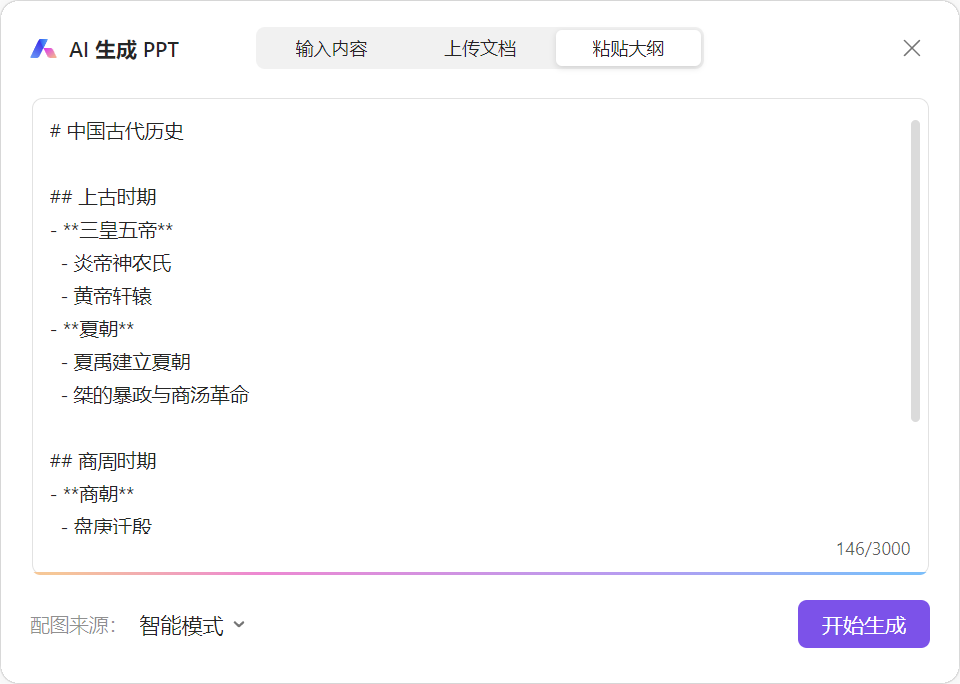
\includegraphics[width=0.7\textwidth]{assets/figures/image-20250210192847219.png} %插入图片,[]中设置图片大小,{}中是图片文件名
      \caption{粘贴大纲到WPS} %最终文档中希望显示的图片标题
      \label{fig:ppt-wps} 
}

\fig[h]{
      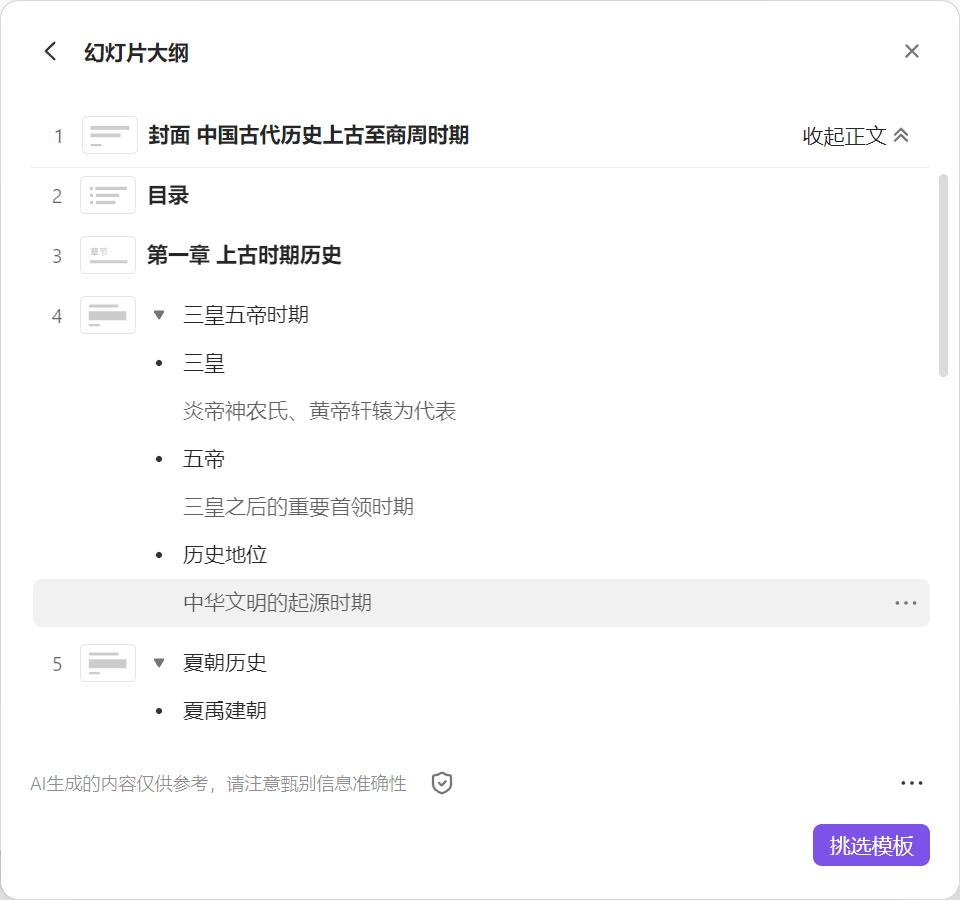
\includegraphics[width=0.7\textwidth]{assets/figures/image-20250210192936323.png} %插入图片,[]中设置图片大小,{}中是图片文件名
      \caption{WPS生成大纲} %最终文档中希望显示的图片标题
      \label{fig:ppt-wps-toc} % 
}

\fig[h]{
      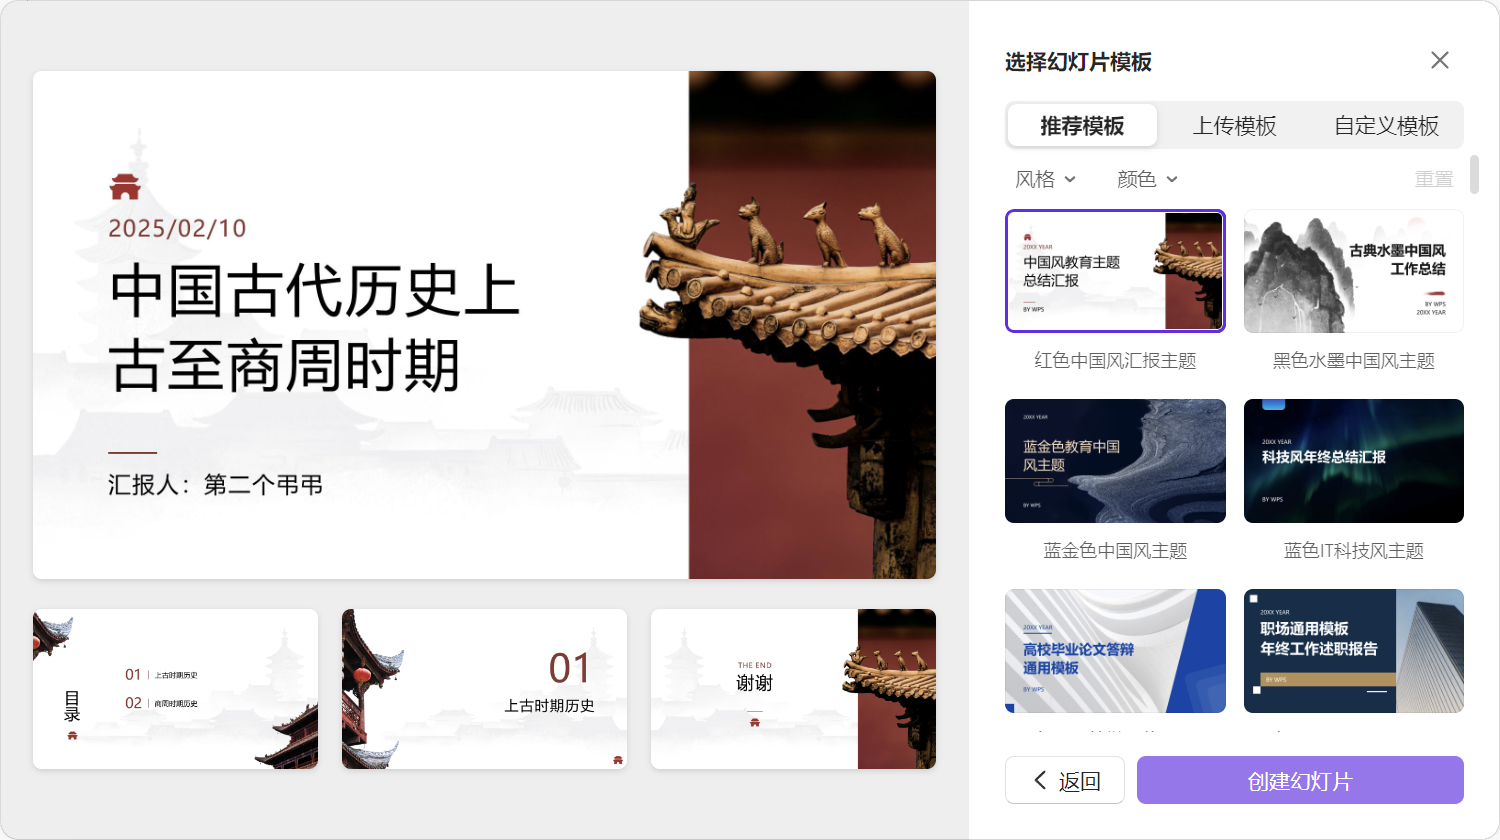
\includegraphics[width=0.7\textwidth]{assets/figures/image-20250210192952252.png} %插入图片,[]中设置图片大小,{}中是图片文件名
      \caption{挑选合适的模板} %最终文档中希望显示的图片标题
      \label{fig:ppt-wps-select} % 
}

\fig[h]{
      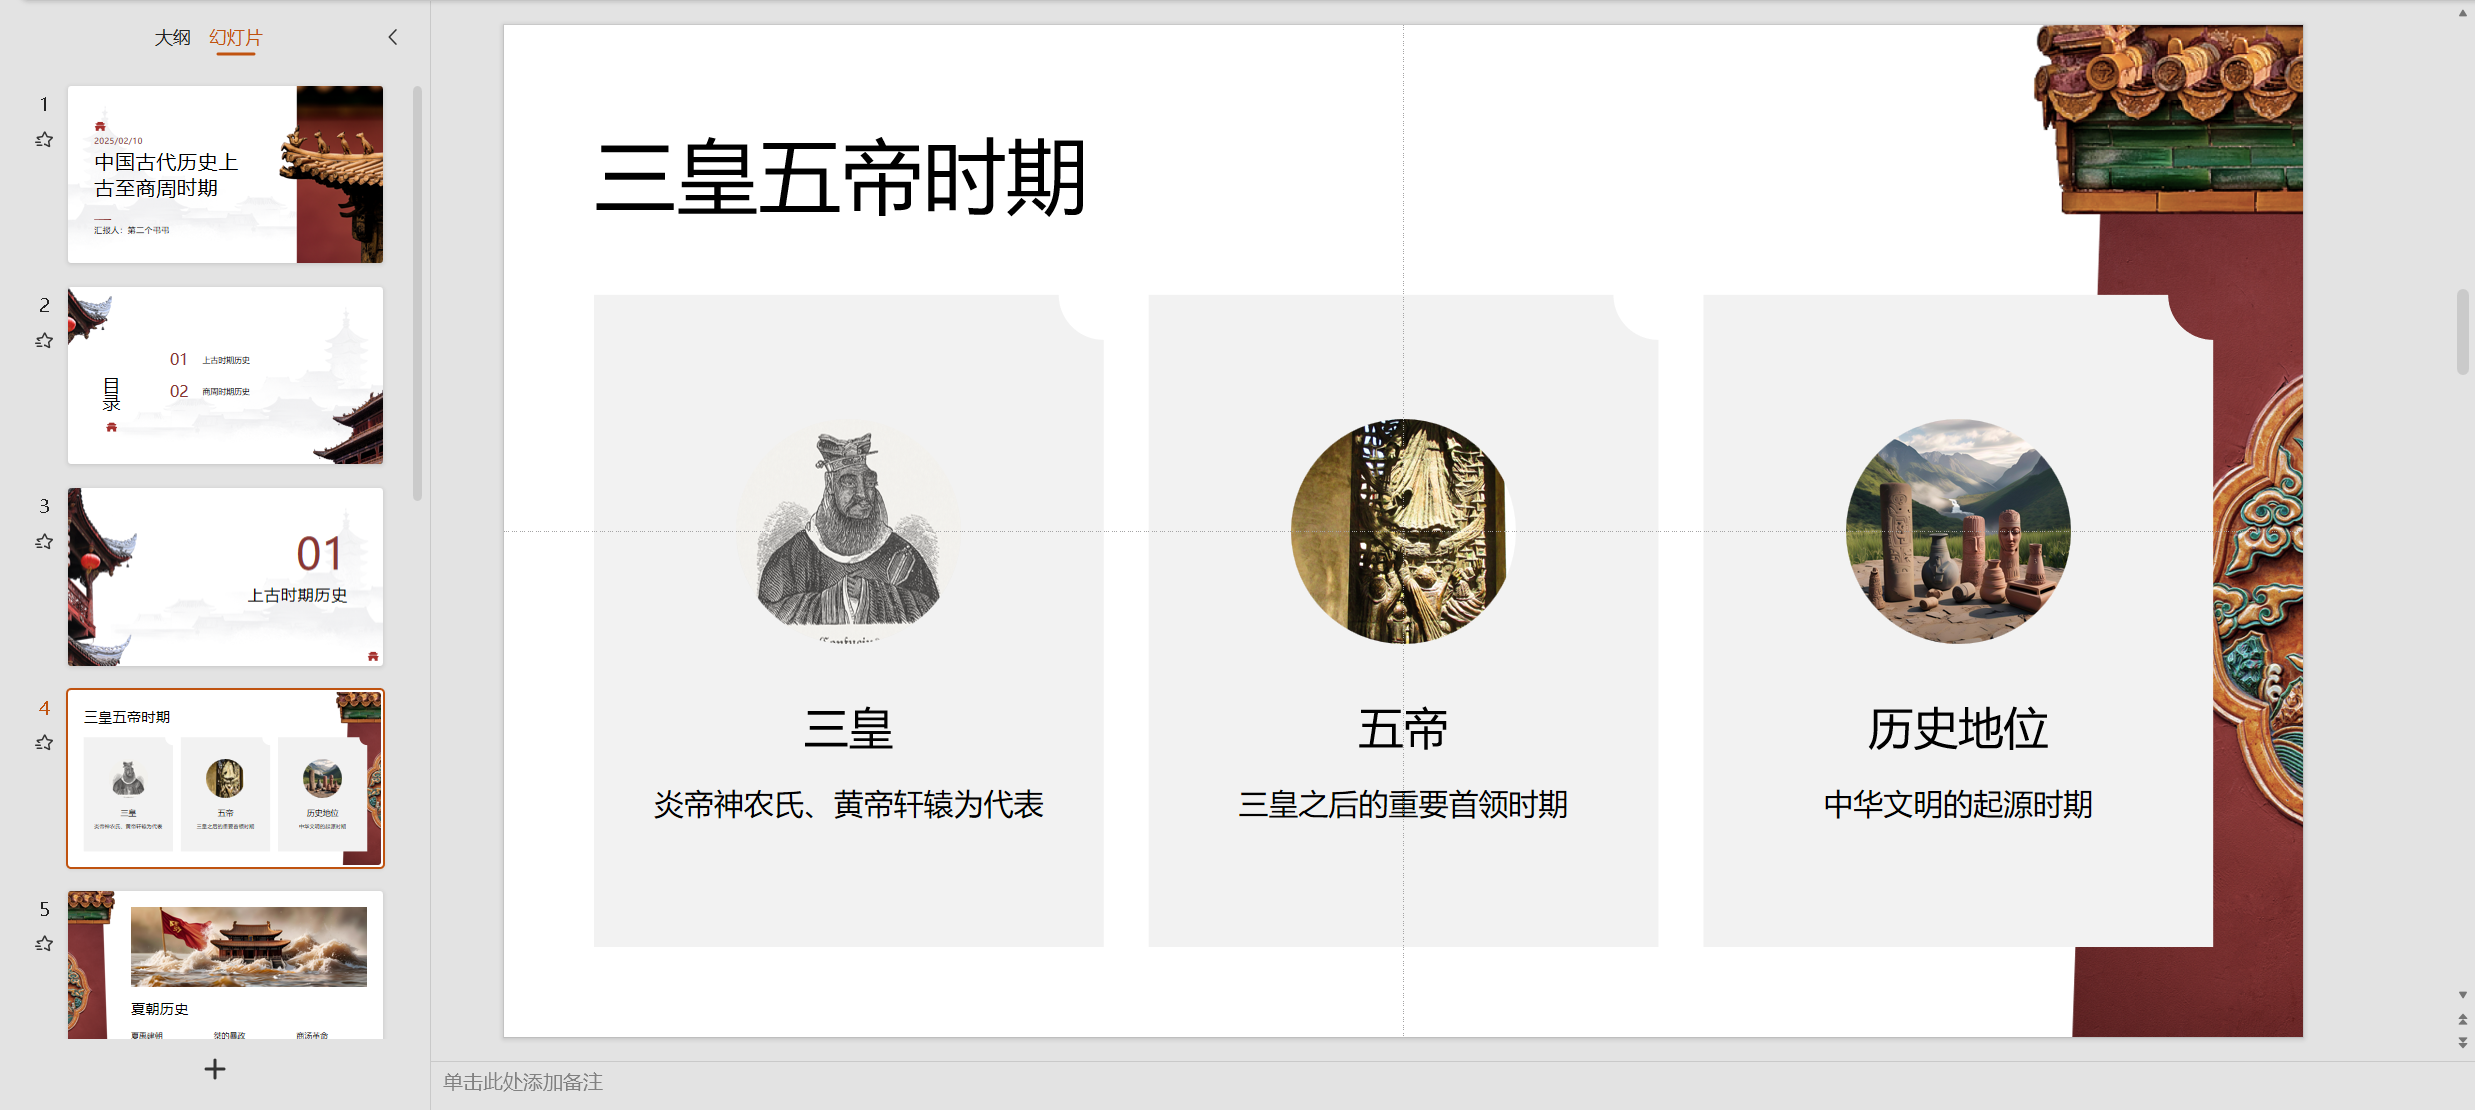
\includegraphics[width=0.7\textwidth]{assets/figures/image-20250210193018631.png} %插入图片,[]中设置图片大小,{}中是图片文件名
      \caption{效果图} %最终文档中希望显示的图片标题
      \label{fig:ppt-wps-done} %用于文内引用的标签 
}

\textbf{步骤四:美化与调整}。在制作历史主题的PPT时,视觉元素的运用对于增强信息的传达效果至关重要。例如,可以通过添加历史地图或重要人物画像,为观众提供直观的历史背景和人物形象,从而加深对历史情境的理解。此外,使用时间轴来展示各个朝代的更替,能够清晰地呈现历史发展的脉络,帮助观众更好地把握历史事件的时间顺序和相互关系。同时,在关键事件的页面中加入简短的动画效果,不仅可以吸引观众的注意力,还能通过动态呈现增强其对复杂历史过程的理解和记忆。这些设计手段不仅丰富了PPT的视觉效果,更在学术表达上提升了内容的可读性和教育价值。

综上,通过GPT生成结构化的内容,并结合专业的PPT制作工具,我们可以高效地创建出内容丰富、设计美观的历史PPT。这种方法不仅节省时间,还能确保信息的准确性和呈现的专业性,特别适合文科生在学习和教学中使用。随着技术的发展,未来的工具将更加智能,帮助我们更轻松地完成复杂的任务。

值得一提的是,在运用GPT生成历史相关内容时,常会面临一些关键性问题,而这些问题的妥善解决对于保证学术性和教学效果至关重要。首先,关于内容的准确性问题,尽管GPT具备强大的信息生成能力,但在处理历史知识时,仍需谨慎对待。历史学科的严谨性要求我们在使用生成的内容后,必须进行仔细的校对,并参考权威的历史资料加以验证。通过这一过程,可以有效避免因技术生成的偏差而带来的错误信息,确保内容的科学性和可靠性。
其次,面对复杂的主题,如何有效处理也是一个重要问题。历史学科中不乏内容丰富且层次复杂的主题,如某一历史时期的变革或某一重大事件的多维度影响。在这种情况下,可以采用分步查询的方法,逐步向GPT提出细化的问题,从而逐步完善每个部分的内容。通过这种方式,能够确保在生成内容时,结构清晰、逻辑连贯,避免因内容过于庞杂而导致的混乱。这种分步细化的策略不仅有助于提高内容的质量,也使得历史知识的呈现更加条理化,便于学习者理解和接受。

% \section{AI配音}\label{sec:dubbing}
在数字化信息高速发展的时代,信息传播的形式愈发多元。配音在众多场景中都有着举足轻重的作用。对于内容创作者而言,无论是制作教育视频、有声读物,还是科普短视频,优质的配音都能极大地增强内容的吸引力与感染力。

在教育领域,这一需求尤为突出。例如,在制作教学 PPT 时,不少教师因自身声音条件不够理想,或者普通话不够标准,导致讲解效果大打折扣。而 GPT 辅助配音就能很好地解决这些问题。它可以为 PPT 配上清晰、标准且富有感染力的语音讲解,让学生更专注于知识内容本身,提升学习效果。

又如在网课制作中,教师可能会遇到语言转换的难题。当需要将中文课程内容转化为英文讲解,以满足不同学生的学习需求时,传统方式不仅复杂,还容易出错。而借助 GPT 辅助配音,能够轻松实现汉语转英语、英语转汉语的配音操作,极大地拓展了课程的受众范围,让知识得以跨越语言障碍传播。

此外,在制作有声读物时,生动的配音能让听众仿佛身临其境,沉浸在故事的世界里。但传统的人工配音往往面临成本高、周期长的问题,特别是对于预算有限的创作者或小型团队来说,难以承担高昂的配音费用。此时,GPT 辅助配音就成为了极具吸引力的解决方案。


利用 GPT 辅助配音的过程相对简便。首先,要准备好待配音的文本内容,它可以是一段课程讲解文案、一篇故事文稿,亦或是 PPT 中的文字内容。将这些文本输入到支持 GPT 技术的配音平台中,平台基于 GPT 强大的语言理解和生成能力,对文本进行深度分析。它会精准识别文本中的情感基调、重点词汇等关键信息。例如,如果文本是一段欢快的儿童故事,GPT 会根据词汇和语句结构判断出需要以活泼、轻快的语调进行配音;若是一篇严肃的学术报告,配音则会偏向沉稳、专业。
然后,平台会从众多预设的配音风格和音色库中,挑选出最适合文本的配音方案,生成相应的音频文件。在整个过程中,用户还能根据自身喜好对语速、音量等参数进行微调,以达到最满意的效果。比如,教师在为网课配音时,可以根据教学节奏,适当调整语速,突出重点内容。



GPT 辅助配音带来了诸多好处和优势。从成本角度来看,它大大降低了配音成本,无需支付高昂的人工配音费用,为广大创作者节省了资金。在效率方面,传统人工配音可能需要预约配音演员、安排录制时间等,整个流程耗时较长,而 GPT 辅助配音能在短时间内完成配音工作,极大地提高了创作效率。在灵活性上,用户可以随时根据自己的需求对配音进行修改和调整,不受时间和空间的限制,而人工配音修改起来则相对繁琐。
尤其是在教育教学场景中,GPT 辅助配音能够克服教师自身声音和语言方面的不足,实现多语言配音转换,让知识传播更加广泛和高效。与原始的人工配音方法相比,GPT 辅助配音以其低成本、高效率、高灵活性的特点,为内容创作领域,特别是教育内容创作带来了新的活力,成为众多创作者在配音需求上的理想选择。

下面以讯飞星火\footnote{\url{https://xinghuo.xfyun.cn}}为例探究如何使用AI进行配音。
\textbf{步骤一:}进入科大讯飞官网,注册并登录账号。
\textbf{步骤二:}点击智能体中心,搜索配音,选择配音员(也可根据需求选择其他配音功能,如:文字转语音大师、短视频脚本等等)。
\textbf{步骤三:}输出需要配音的内容。
最后与AI的对话展示如下:

\prompt{请生成音频:我是中国人}

\begin{gptbox}
\footnotesize{
    \textbf{[已生成音频文件]}

    \textbf{“我是中国人”声音处理分析}

    “我是中国人”这句话虽简短,但通过细致的声音处理,可传达出深厚情感和自豪感。以下是详细分析:

    \textbf{一、逐字分析与声音表现}
    \begin{enumerate}
        \item \textbf{每个字的发音细节}
              \begin{enumerate}
                  \item \textbf{我}:
                        音调可适当用稍低、沉稳的音调起头,如中央C下方的A音(实际演唱中可根据个人音域调整),营造庄重、严肃氛围开场,体现坚定的自我认知和身份认同。
                        音量起始不宜过大,以轻柔、适中音量发声,像在安静诉说重要事实,给听众亲切又稳重之感。
                        节奏微微拖长一点音,时值大概是正常说话节奏的1.2 - 1.5倍,强调主体,吸引听众注意力。
                  \item \textbf{是}:
                        紧接着“我”之后,音调轻微上扬,从A音上滑到B音左右(按简谱大致示意),起过渡和衔接作用,暗示确认、肯定语气。
                        音量相较于“我”稍加强一点,保持在中等偏下适度音量范围,突出连接词重要性,使表达更连贯。
                        节奏正常节奏稍快一点说出,干脆利落表明身份归属关系。
                  \item \textbf{中国}:
                        “中”字发音从中等的G音起,平稳过渡到“国”字的高音A音(简谱示意),“国”字适当延长音调并保持稍高的音值,体现对国家名称的尊崇与敬意,凸显自豪感。
                        音量说到“中国”时明显增强,达句子音量峰值,以饱满、洪亮声音喊出,传递强烈爱国情怀。
                        节奏放缓,“国”字时值拖长到正常说话节奏的1.5 - 2倍,突出“中国”,强化民族归属感和认同感。
                  \item \textbf{人}:
                        最后落在“人”字,音调从“国”字较高的A音平稳下降到G音左右(简谱示意),回归平稳、踏实,带着对所属群体的亲切和归属感。
                        音量较“中国”稍弱,但仍保持较强程度,维持坚定有力气势。
                        节奏正常节奏收尾,利落干脆结束句子讲述。
              \end{enumerate}
        \item \textbf{词与词之间的联系、抱团或停顿}
              \begin{itemize}
                  \item \textbf{联系}:“我”“是”“中国人”紧密相连,构成完整身份表述,存在逻辑因果关系,需通过声音连贯性体现内在联系。
                  \item \textbf{抱团}:“中国”两字抱团处理,发音一气呵成,作为整体概念,避免歧义或破坏表达完整性。
                  \item \textbf{停顿}:“我是”后面可有0.2 - 0.3秒左右极短停顿(具体时长可根据整体语速和个人风格微调),像个小缓冲,便于讲述者和听众转换情绪、理解内容,为强调“中国人”做铺垫;句子结尾处有0.5 - 0.8秒稍长停顿,给句子完整结束感,让听众回味情感与意义。
              \end{itemize}
        \item \textbf{音调的变化(走低或渐扬)}

              整体音调呈现先抑后扬再平稳趋势。开头“我”字音调稍低营造庄重氛围;“是”字小上扬过渡;“中国”音调上扬并保持较高位置突出重点;“人”字平稳下降回归自然。这种音调变化如山峰起伏,吸引听众注意力,传达讲述者复杂情感变化,从自我认知出发,经对国家崇敬热爱的高潮表达,最后落到对所属群体的亲切认同,增强句子表现力和感染力。
    \end{enumerate}
}
\end{gptbox}



% \section{AI生成式绘画}\label{sec:painting}
在绘画领域,GPT不仅为创作者提供了强大的技术支持,还通过其生成能力,极大地拓展了绘画创作的边界。它能够实现多种复杂的图像操作,从生成创意草图到辅助完成细节绘制,为艺术家们提供了全新的创作思路和工具。这种技术与艺术的深度融合,不仅推动了绘画创作方式的变革,也为艺术表现形式带来了前所未有的可能性,进一步丰富了当代艺术的内涵与外延。

利用 GPT 的图像超分辨率技术,可以将低分辨率(1k)的图像无损地提升至高分辨率(4k)。这一过程通过深度学习算法对图像中的细节进行智能补充和重建,使得原本模糊的图像变得更加清晰锐利,满足对高清图像的需求,比如在印刷、大型展示等场景下的应用。GPT 可以精准识别图像主体与背景,通过算法自动去除背景,留下干净的主体图像。这对于需要将主体单独提取出来用于合成、设计等工作非常方便,大大节省了手动抠图的时间和精力。只需简单的指令,GPT 就能将图像的颜色进行反转,即黑变白、白变黑,其他颜色也相应反转。这种操作在一些创意设计、艺术创作中能带来独特的视觉效果,也有助于图像分析等工作。
当图像存在噪点影响视觉效果时,GPT 能够运用其去噪算法,智能识别并去除噪点,使图像恢复清晰、平滑,提升图像质量。用户可以向 GPT 输入想要替换的背景描述,如 “将当前图像背景替换为蓝天白云的草原场景”,GPT 会根据描述生成新的背景,并与原图像主体完美融合,创造出全新的画面效果。同样,若要替换图像中的人物,只需提供新人物的特征描述,如 “将画面中的人物换成一位穿着古装的女子”,GPT 就能完成人物替换,同时保证整体画面的协调性和逻辑性。无论是想要一张科幻风格的城市夜景图,还是温馨的家庭生活场景图,只要给出详细的需求,如 “生成一张未来城市中飞行汽车穿梭的图片,城市中有绚丽的霓虹灯和高楼大厦”,GPT 就能按照要求生成满足特定需求的高质量图片。GPT 可以根据文本描述生成各种想象中的场景。比如,当输入 “生成一个古代仙侠世界中的神秘山谷,山谷中有清澈的溪流、奇形怪状的石头和盛开的花朵”,它能迅速构建出相应的场景画面,为绘画创作者提供丰富的灵感和基础素材,大大加快创作进程。用户可以指定将一种图像风格迁移到另一种图像上。例如,将梵高的油画风格应用到一张普通的风景照片上,GPT 会分析梵高油画的笔触、色彩特点等,然后将这些风格元素融入到目标图像中,使其具有梵高油画的独特艺术风格。

\subsection{内容生成}

下面以liblib\footnote{\url{https://www.liblib.art}}为例演示AI生成图片的过程。首先在页面中选择合适的模型并输入提示词,该工具会自动将提示词转换为英文,最终得到生成的图片。

\prompt{设计一座未来主义风格的生态城市中心,融合高科技与可持续发展理念。建筑外观采用流线型结构,表面覆盖智能玻璃幕墙,能够根据天气和光线自动调节透明度。建筑内部设有垂直花园和空中花园,以最大化绿化空间。屋顶配备太阳能板和雨水收集系统,以实现能源自给自足和水资源循环利用。整体风格简洁而富有科技感,同时融入自然元素,营造出人与自然和谐共生的未来城市景观。}

\begin{gptbox}
\footnotesize{以下是生成的图片:}
\fig[H]{
    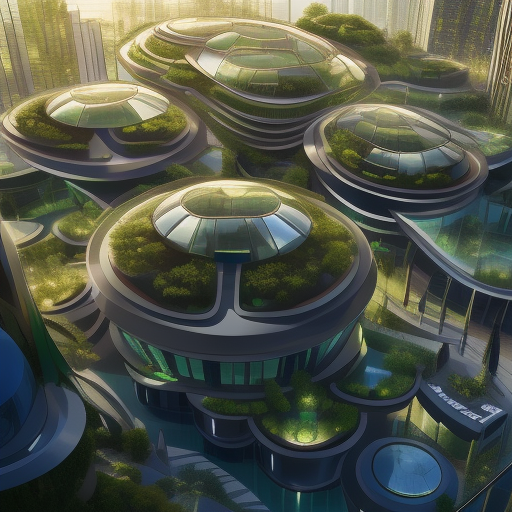
\includegraphics[width=0.7\textwidth]{gc}
}
\end{gptbox}


\subsection{图像风格转移}

在探索人工智能辅助图像编辑的前沿领域时,一个值得关注的工具是InstructPix2Pix。该模型由Hugging Face平台上的开发者timbrooks创建,能够根据用户输入的提示词对图像进行修改和变换,从而实现高度定制化的图像生成。用户可以通过访问InstructPix2Pix - a Hugging Face Space by timbrooks进入该模型的交互界面,如\reffig{fig:gc-InstructPix2Pix}所示。

在使用该工具时,用户首先需要上传待修改的图像,这一操作以红色框标出。随后,用户需在蓝色框中输入提示词,以描述期望的图像修改效果。为确保最佳效果,建议使用英语,并尽可能以简洁明了的方式表达需求。此外,界面中的绿色框提供了参数调整选项,其中“Text CFG”和“Image CFG”是两个关键参数。Text CFG用于调节提示词的权重,而Image CFG则用于调整图像本身的权重。用户可以通过对这两个参数的精细调整来实现预期的图像效果。然而,需要注意的是,这两个参数之间必须保持适当的平衡。如果Text CFG权重过高,可能导致生成的图像与原始图像失真;而如果Image CFG权重过高,则可能使生成的图像无法完全符合提示词的要求。因此,用户在使用过程中需要根据具体需求灵活调整参数,以达到理想的效果。

\fig[h]{
    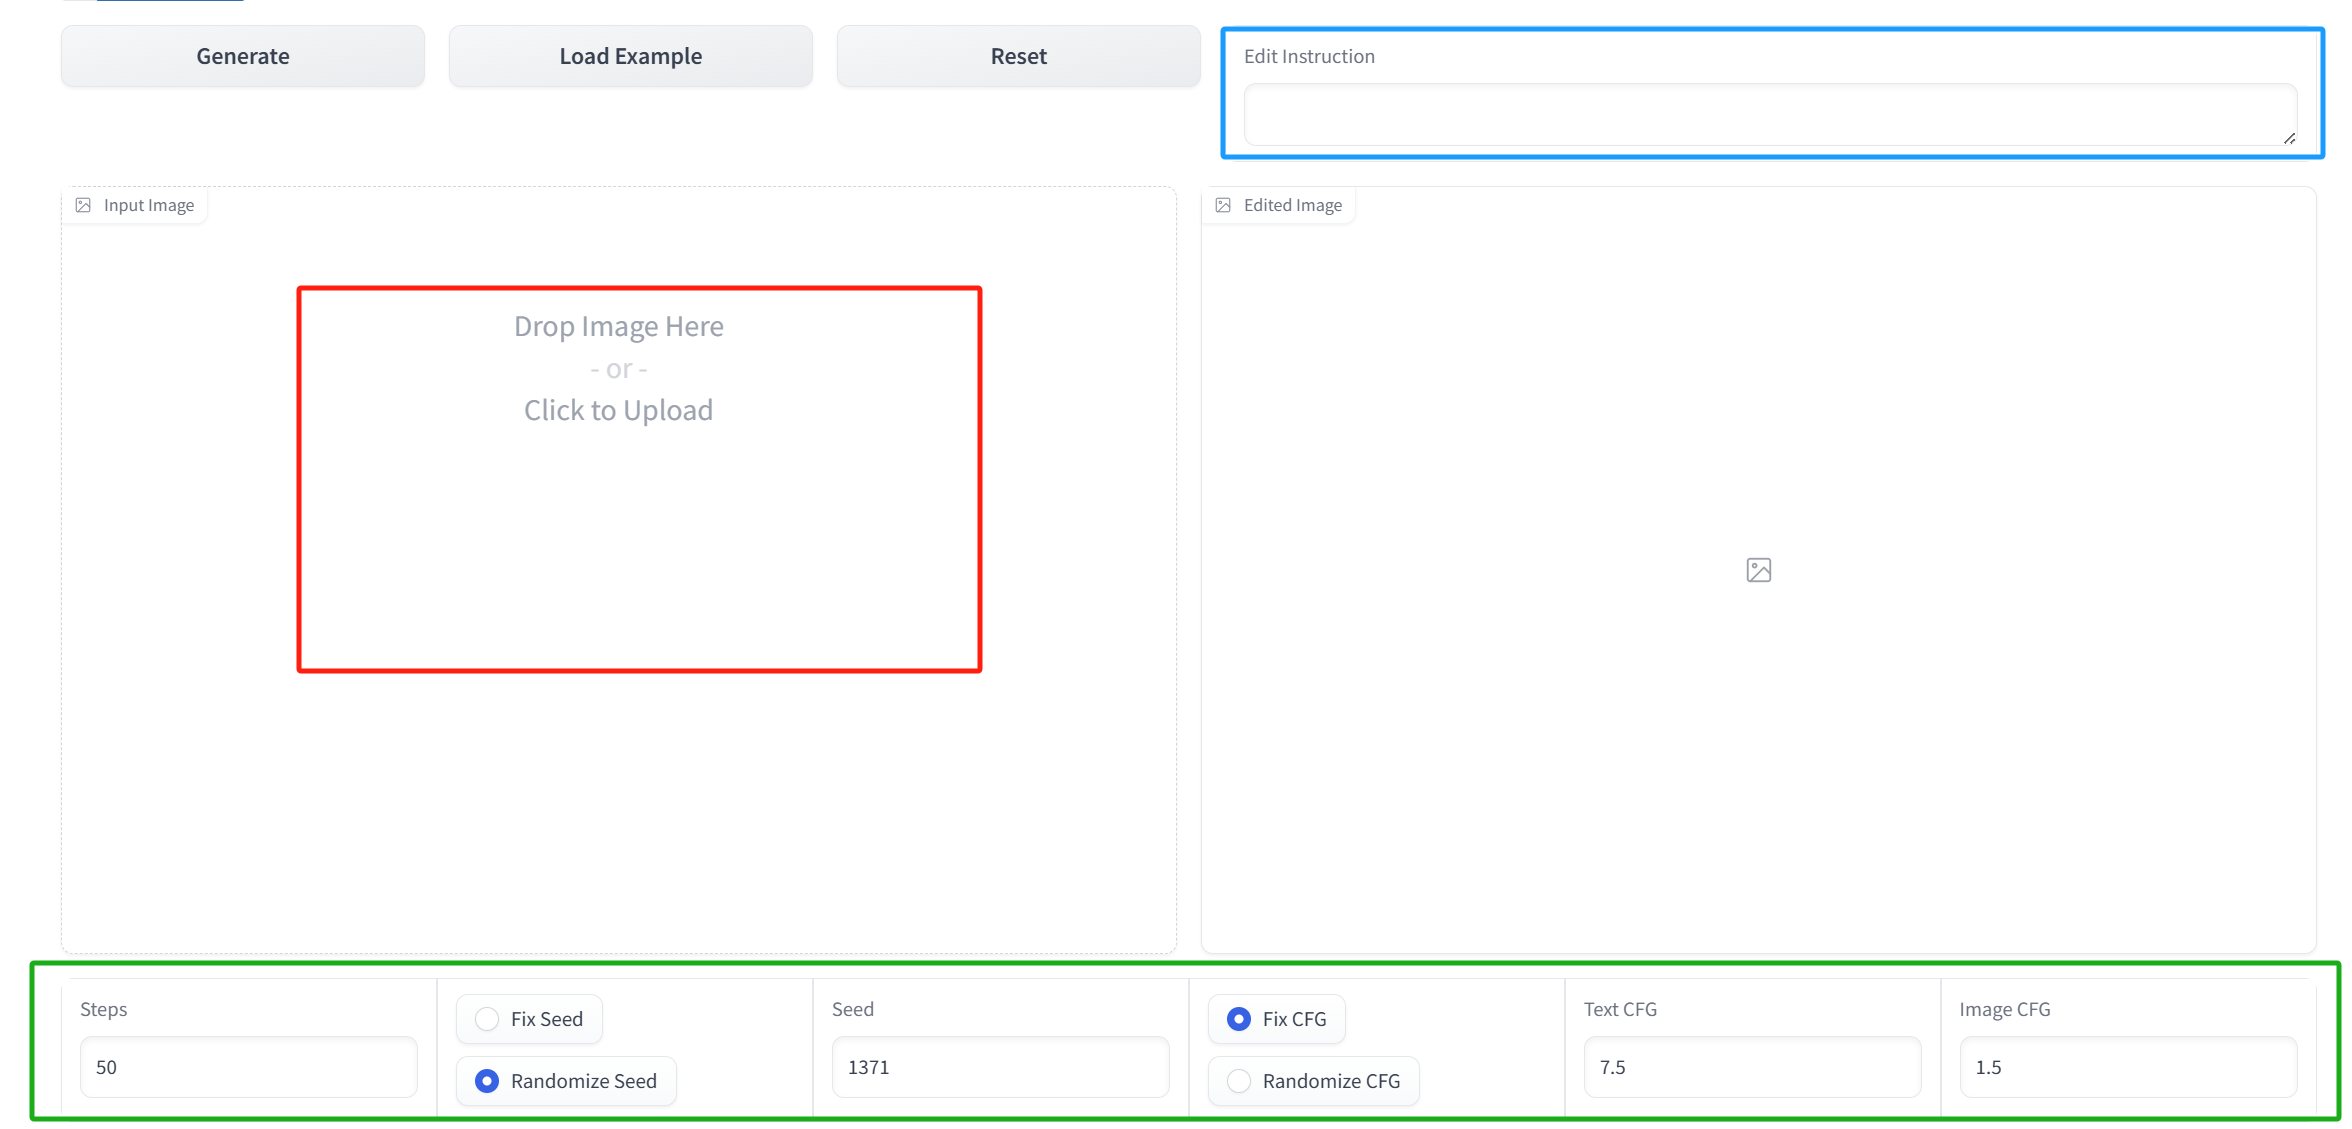
\includegraphics[width=0.7\textwidth]{assets/figures/image-20250211145347208.png} %插入图片,[]中设置图片大小,{}中是图片文件名
    \caption{InstructPix2Pix参数调整} %最终文档中希望显示的图片标题
    \label{fig:gc-InstructPix2Pix} 
}

例如,若需将云南师范大学的校园照片转化为动漫风格,可通过精心设置相关参数并输入恰当的提示词来实现这一风格转换,如\reffig{fig:gc-rendering}和\reffig{fig:gc-rendered}所示。

\fig[h]{
    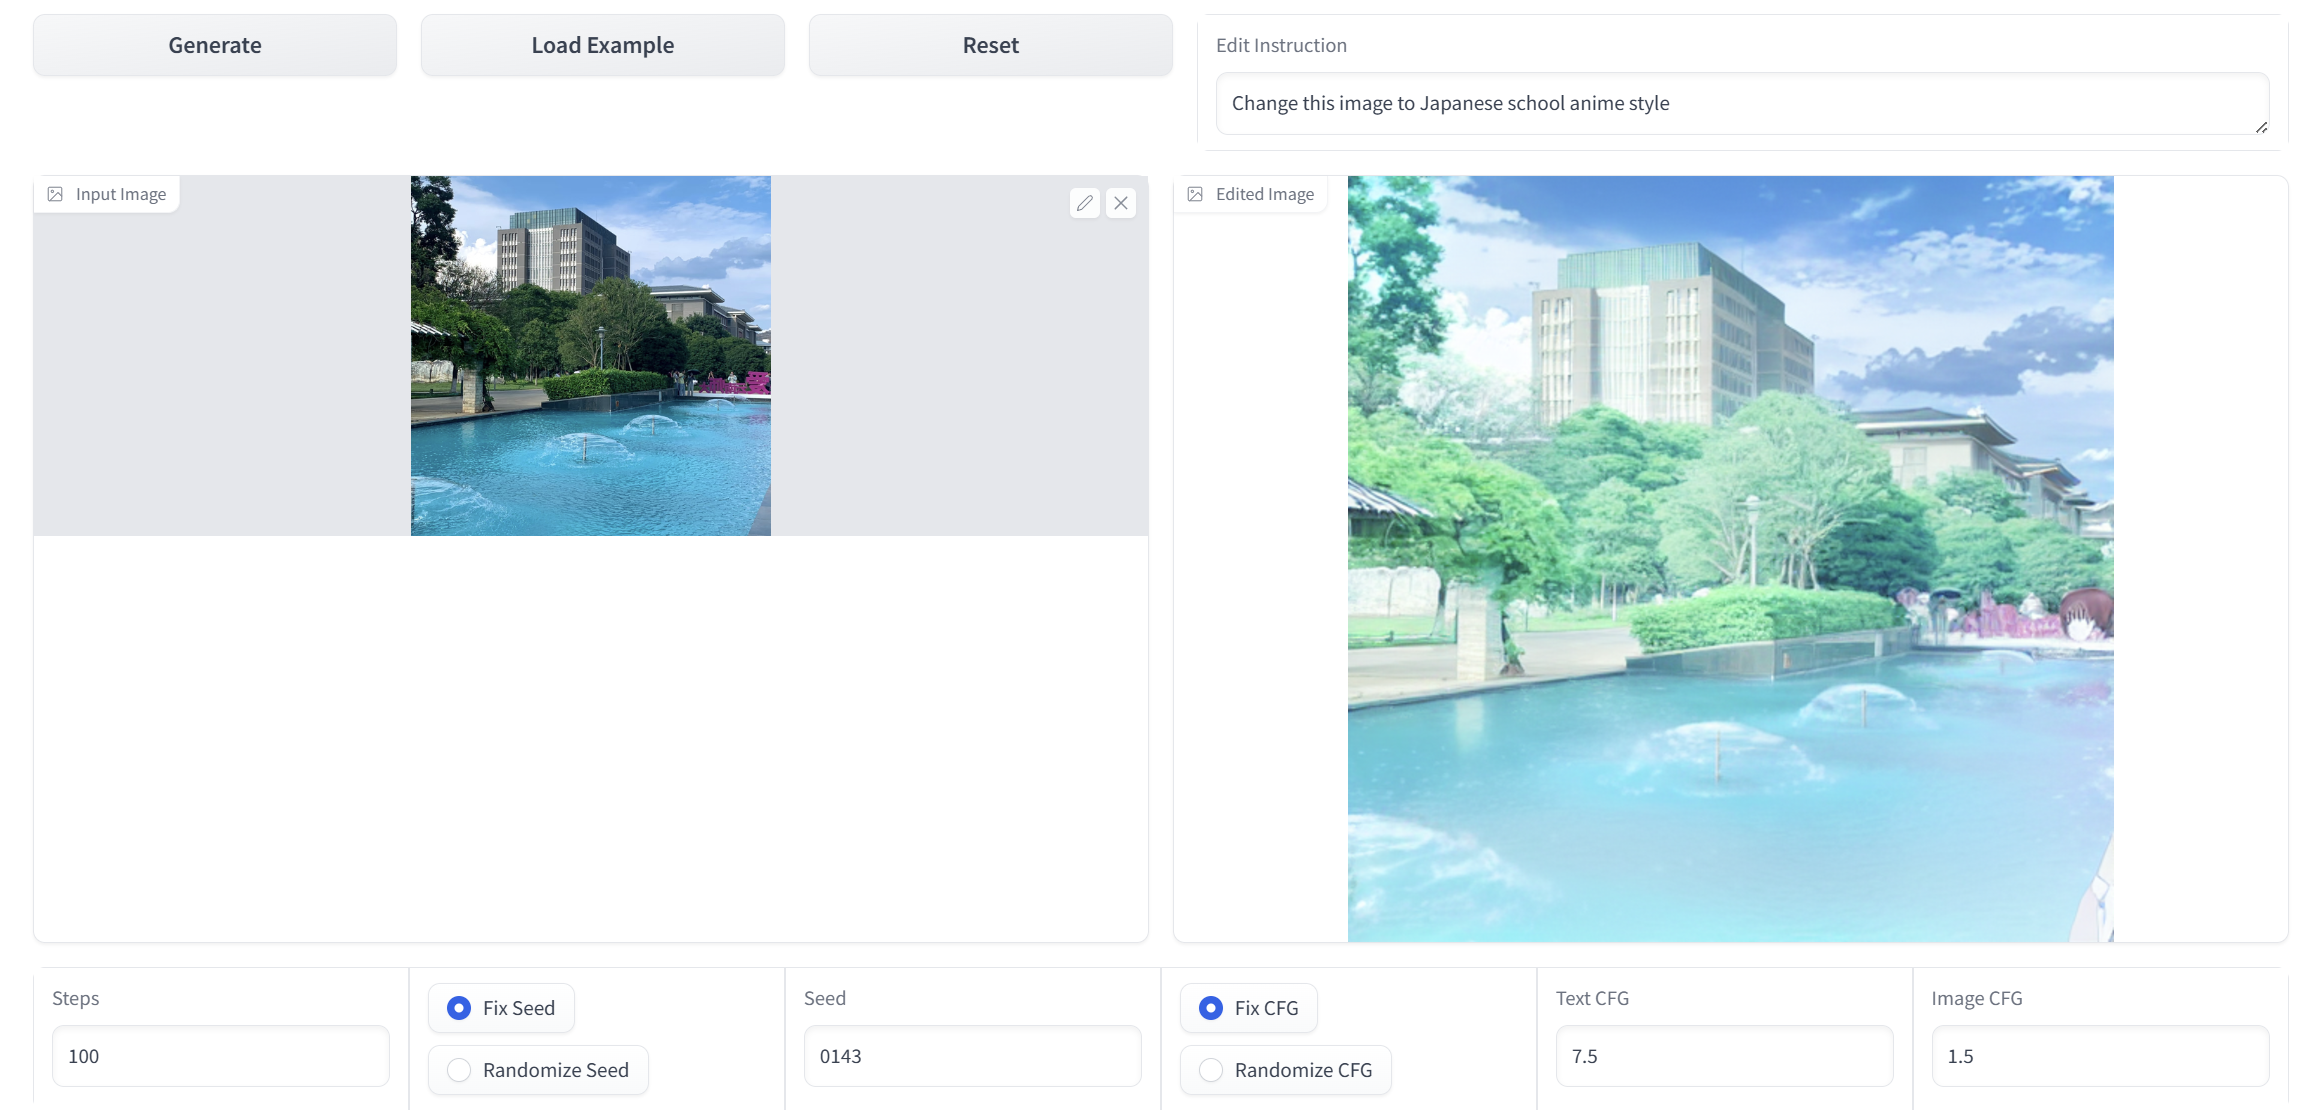
\includegraphics[width=0.7\textwidth]{assets/figures/9c6c2ff0409374eed093b8ec3447507.png} %插入图片,[]中设置图片大小,{}中是图片文件名
    \caption{渲染过程} %最终文档中希望显示的图片标题
    \label{fig:gc-rendering} 
}

\fig[h]{
    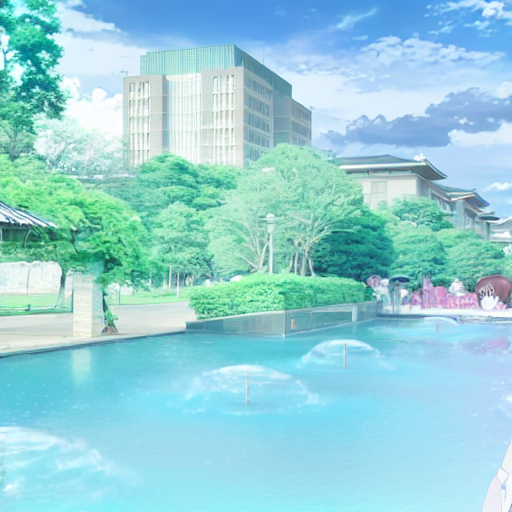
\includegraphics[width=0.7\textwidth]{assets/figures/change.png} %插入图片,[]中设置图片大小,{}中是图片文件名
    \caption{渲染效果图} %最终文档中希望显示的图片标题
    \label{fig:gc-rendered} 
}

通过对比两幅图像,可以清晰地观察到其风格上的显著差异。在此基础上,用户可进一步调整参数,以不断优化并最终实现预期的图像效果。




% \section{AI动画}

在动画领域,人工智能(AI)正以其强大的技术力量掀起一场前所未有的变革。AI动画的出现,不仅是技术的进步,更是艺术创作的一次深刻革命。它利用先进的算法和模型,从角色设计到场景渲染,从动作捕捉到特效生成,全方位重塑了动画制作的流程。

以近期备受瞩目的国产动漫电影《哪吒2》为例,AI技术贯穿了从前期设计到后期制作的全流程。AI辅助设计系统能够快速生成角色概念图,大大缩短了创作周期;AI动作捕捉技术精准记录演员表演,并将其转化为数字角色的动作数据;AI渲染引擎则通过深度学习算法,实现了更加真实的光影效果和材质表现。这种技术的应用不仅提升了制作效率,更突破了传统动画制作的局限,为观众带来了前所未有的视觉体验。

在角色设计方面,AI通过学习大量数据,能够生成符合特定主题或风格的独特角色设计,并实现风格迁移和个性化定制。而在动画制作过程中,AI技术可以自动生成动作和表情,减少人工绘制的工作量,同时利用动态捕捉技术实现更逼真的表现。此外,AI还能自动生成动画中的特效,如烟雾、火焰、水波等,进一步提升视觉效果。

AI动画的崛起,不仅改变了动画的制作方式,更拓展了其应用场景。从教育类动画到广告动画,AI能够根据不同的需求进行个性化定制,满足不同观众群体的偏好。这种高度的灵活性和适应性,使得AI在动画领域的应用前景愈发广阔。

然而,AI动画的发展也带来了新的挑战。一方面,确保生成动画的高质量并非易事;另一方面,传统动画技能可能面临被掩盖的风险。尽管如此,AI与传统动画方法的结合,仍为动画师和内容创作者提供了无限的可能性。随着技术的不断进步,AI动画的未来充满希望,它将继续推动动画产业迈向新的高度。

下面以郑和下西洋为背景,使用AI工具制作一个简单的动画。

\prompt{生成30秒的郑和下西洋动画剧本,包含船队出发、海上航行、异国贸易三个场景}


\begin{gptbox}
s \footnotesize{
  \textbf{《郑和下西洋》动画剧本}

  \textbf{场景一:船队出发}
  \begin{itemize}
      \item \textbf{镜头1:南京城外港口}
      \begin{itemize}
          \item \textbf{画面}:清晨,南京城外港口,宝船队整齐排列,旗帜飘扬,人群欢呼。
          \item \textbf{旁白}:公元1405年,郑和奉命下西洋,船队从南京出发,开启伟大征程。
          \item \textbf{音乐}:激昂的古风音乐,带有海浪声。
      \end{itemize}
  \end{itemize}
  
  \textbf{场景二:海上航行}
  \begin{itemize}
      \item \textbf{镜头2:海上航行}
      \begin{itemize}
          \item \textbf{画面}:船队在波涛中前行,海浪翻腾,船员们忙碌操作。
          \item \textbf{旁白}:船队穿越惊涛骇浪,凭借罗盘和星图,勇往直前。
          \item \textbf{音乐}:紧张的鼓点声,模拟航行的艰难。
      \end{itemize}
  \end{itemize}
  
  \textbf{场景三:异国贸易}
  \begin{itemize}
      \item \textbf{镜头3:异国港口}
      \begin{itemize}
          \item \textbf{画面}:船队抵达异国港口,当地居民热情迎接,贸易市场热闹非凡。
          \item \textbf{旁白}:郑和与各国通商,传播友谊,带回珍宝。
          \item \textbf{音乐}:欢快的异域风情音乐,营造繁荣氛围。
      \end{itemize}
  \end{itemize}
}
\end{gptbox}

% Generate a 10-second animated short film on the theme of “Zheng He's Voyages to the Western Seas,” including the following three scenes: Departure of the Fleet: Depict the grand scene of Zheng He's fleet setting sail from the port outside Nanjing during the Ming Dynasty.Sea Voyage: Show the fleet navigating through the stormy seas, overcoming challenges in a tense sequence. Foreign Trade: Present the fleet arriving at a foreign port and engaging in prosperous trade with the local people in a friendly manner. The script should be concise and highlight the core plot and atmosphere of each scene, suitable for quick storytelling.

接着使用AI视频生成工具清影\footnote{\url{https://chatglm.cn}},使用上述剧本作为提示词得到视频,如\reffig{fig:anime-video}所示。

\fig[h]{
    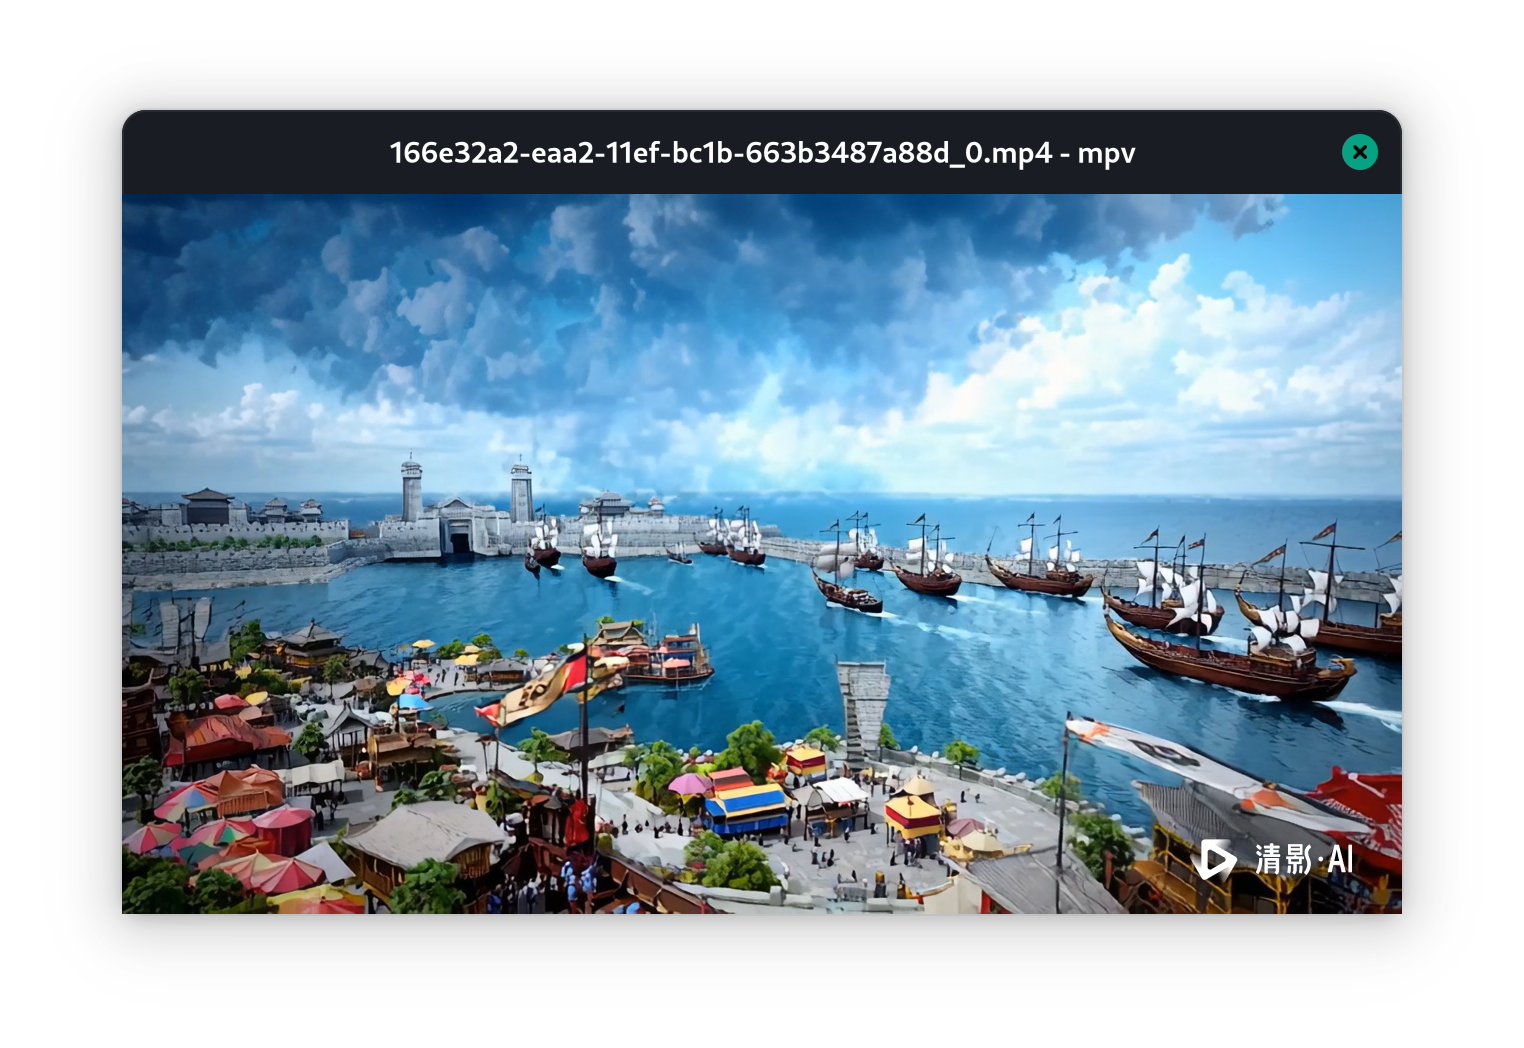
\includegraphics[width=0.7\textwidth]{gc-video}
    \caption{视频结果}
    \label{fig:anime-video}
}

% \section{AI流程图}


AI帮助绘制流程图具有重要意义。它不仅能够显著节省时间,还能提升绘制的准确性和效率。通过自然语言描述,AI工具可以快速生成流程图的基本框架,用户只需输入简单的指令,如“开始”“决策点”“流程步骤”等,AI就能自动识别并绘制相应的图形和连接线。此外,AI还能根据上下文智能识别关键节点和流程关系,即使用户提供的信息不完整,也能推测出合适的步骤。AI工具还能自动调整图形布局和连接线,使流程图更加整洁美观,同时支持实时更新与修改,确保流程图的连贯性和一致性。这种智能化的绘图方式不仅适用于企业管理、项目规划、技术开发等复杂场景,还能帮助个人高效地制定学习计划或整理思维导图,极大地提升了工作效率和质量。


\textbf{案例:历史进程流程图}。本案例旨在梳理``丝绸之路文化交流''中的技术传播路径。下面给出与AI交流过程。

\prompt{``用Mermaid语法绘制佛教从印度经中亚传入中国的流程图,包含主要节点和传播方式''}
  
\begin{gptbox}
\small{
\begin{lstlisting}
graph LR
 A[印度那烂陀寺] -->|法显陆路取经| B[龟兹]
 B --> C[敦煌莫高窟]
 A -->|海上丝绸之路| D[广州光孝寺]
 C --> E[长安大雁塔]
 D --> E
\end{lstlisting}
}
\end{gptbox}


最后,将代码粘贴至Markdown编辑器或Mermaid Live Editor,立即生成矢量图,如\reffig{fig:flow-chart}所示。

\fig[h]{
    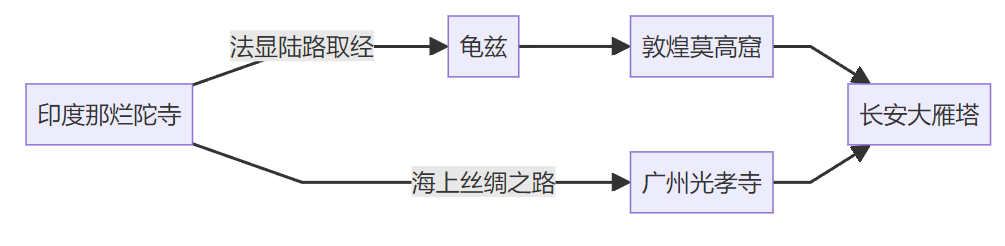
\includegraphics[width=0.7\textwidth]{assets/figures/1739189207681.jpg} %插入图片,[]中设置图片大小,{}中是图片文件名
    \caption{矢量图} %最终文档中希望显示的图片标题
    \label{fig:flow-chart} %用于文内引用的标签
}
\end{enumerate}
% \section{AI辅助3D建模}


AI在3D建模中的应用,如同为创意插上了科技的翅膀,为设计领域带来了前所未有的变革。它不仅极大地提升了建模效率,还为设计师们提供了更广阔的创作空间。借助AI,即使是复杂的3D模型也能在短时间内生成,大大减少了传统手工建模所需的繁琐步骤和时间成本。AI的智能算法能够根据简单的描述或图像快速生成高质量的模型框架,并自动优化结构和纹理,确保模型的精确度和美观度。这种技术不仅降低了3D建模的门槛,让非专业人士也能轻松上手,还能在游戏开发、影视制作、建筑设计、产品设计等多个领域快速响应需求变化,节省大量时间和成本。未来,随着AI技术的不断发展,其在3D建模中的应用将更加广泛,有望为创意产业带来更多的创新和变革,为设计师们提供更强大的工具,推动整个行业的发展。


\textbf{案例:基础3D建模}

本案例通过AI工具快速实现Blender软件中的3D场景原型搭建,为不用3D建模的读者提供快速上手的可能。下面给出与AI工具的交互的过程,可在Blender软件中生成红色正方体,如\reffig{fig:3d-red-cube}所示。

\prompt{写Blender Python脚本:创建一个简单立方体,包含基础灯光和摄像机}


\begin{gptbox} 
\small{ 
\begin{lstlisting}[language=Python] 
import bpy

# 清空场景
bpy.ops.object.select_all(action='SELECT')
bpy.ops.object.delete(use_global=False)

# 创建立方体
bpy.ops.mesh.primitive_cube_add(
    size=2,                # 立方体边长
    location=(0, 0, 0),    # 中心位置
    rotation=(0, 0, 0)     # 初始旋转
)
cube = bpy.context.object
cube.name = "Simple_Cube"  # 命名对象

# 创建基础材质
material = bpy.data.materials.new(name="Cube_Material")
material.diffuse_color = (0.8, 0.1, 0.1, 1)  # RGBA红色
cube.data.materials.append(material)

# 设置摄像机
bpy.ops.object.camera_add(
    location=(5, -5, 3),   # 摄像机位置
    rotation=(1.047, 0, 0.785)  # 60度俯角,45度偏角
)
bpy.context.scene.camera = bpy.context.object

# 添加灯光
bpy.ops.object.light_add(
    type='POINT',
    location=(3, -3, 5),
    radius=1.0
)
bpy.context.object.data.energy = 500  # 灯光强度

# 设置渲染基础参数
bpy.context.scene.render.resolution_x = 1280
bpy.context.scene.render.resolution_y = 720

print("基础立方体场景创建完成!")

\end{lstlisting}
} 
\end{gptbox}

\fig[h]{
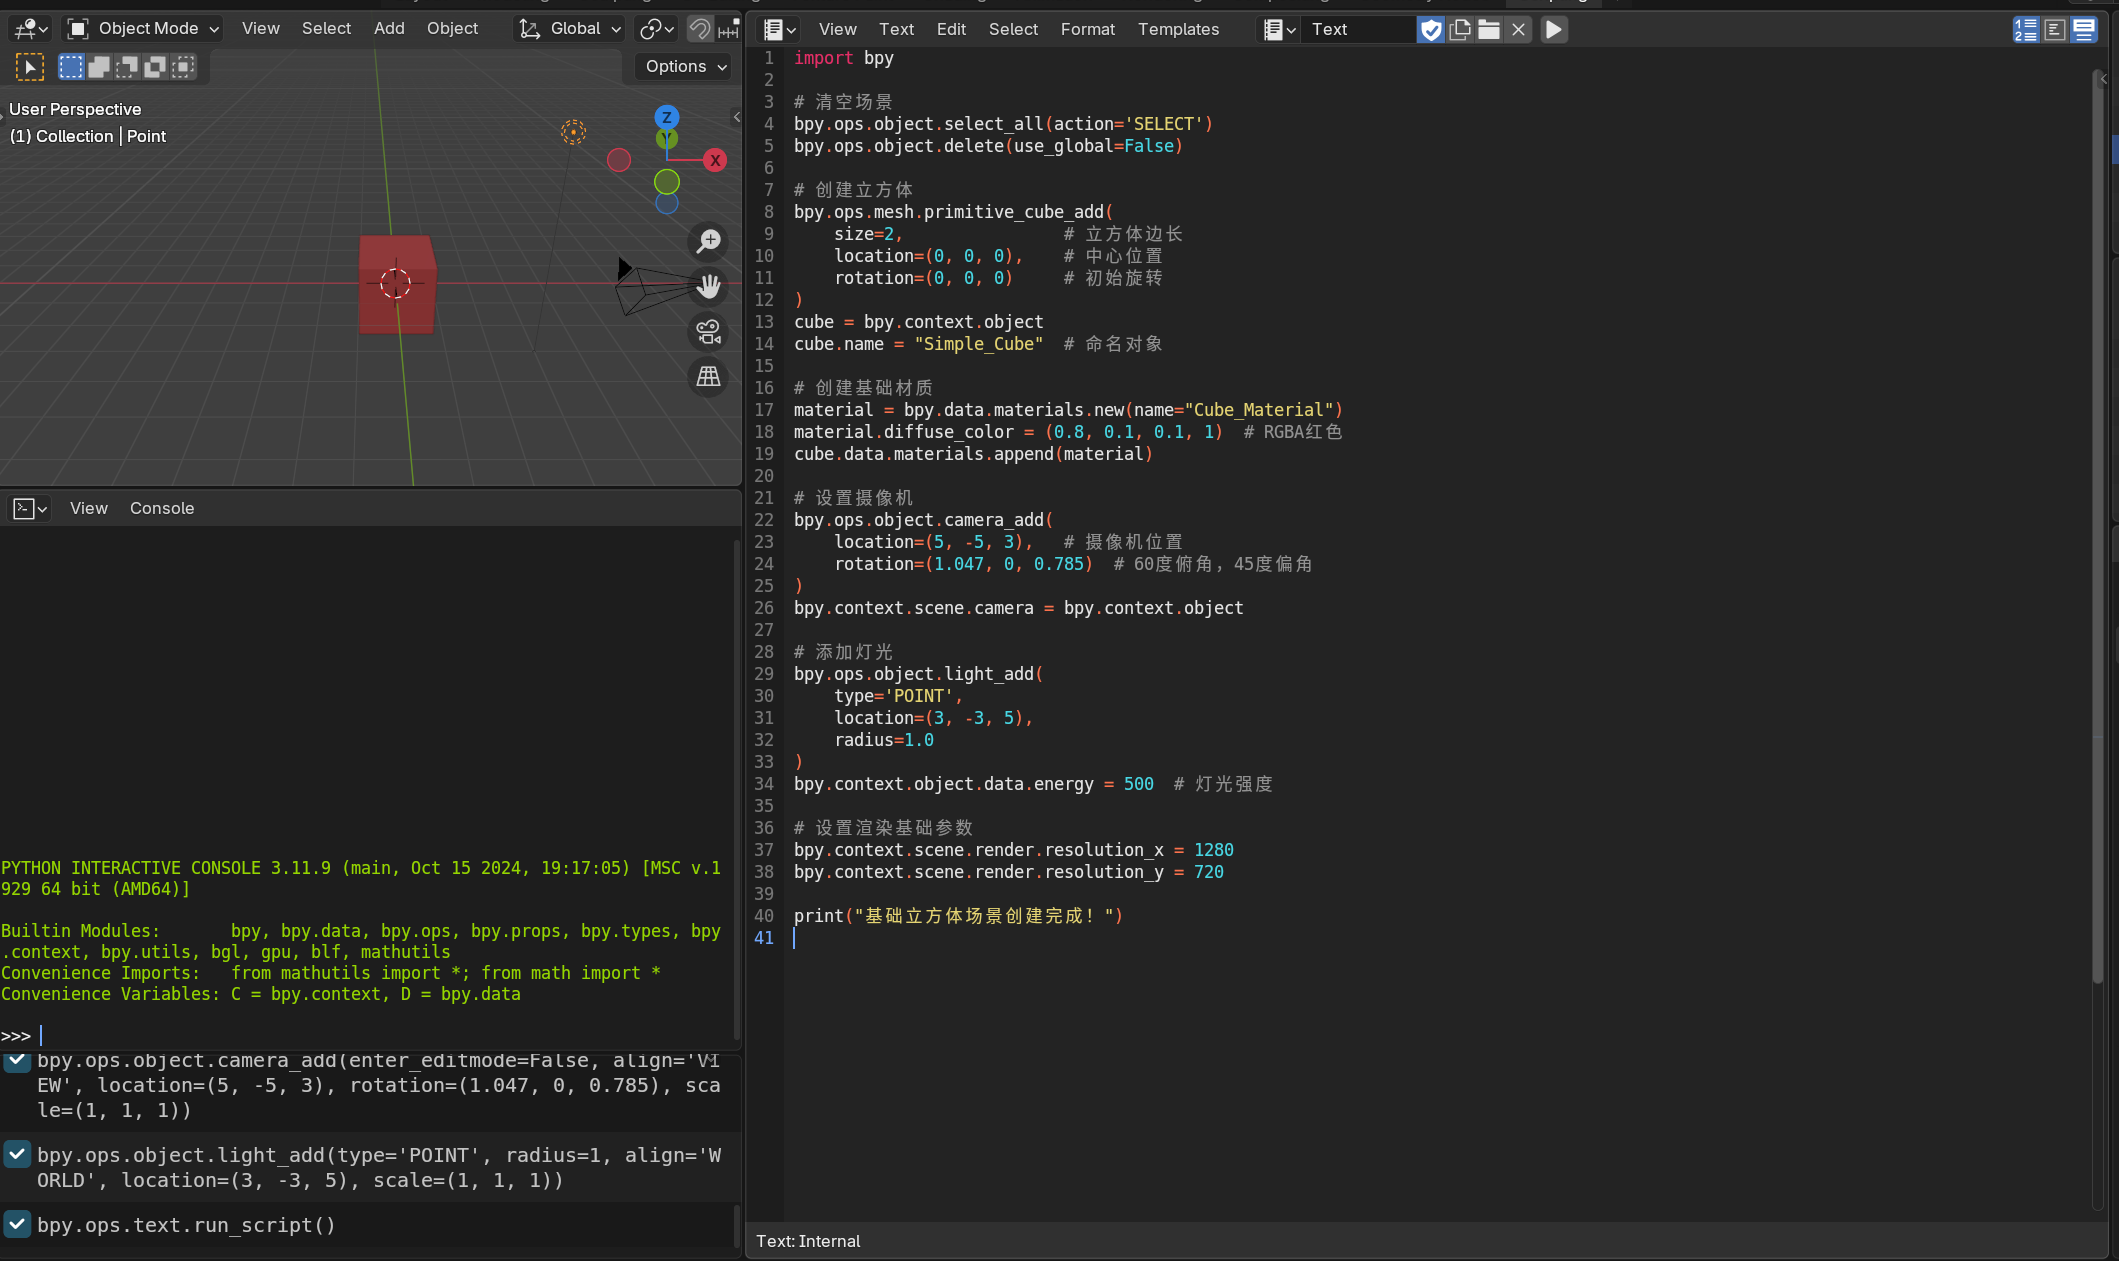
\includegraphics[width=0.7\textwidth]{assets/figures/红色立方体效果图.jpg} %插入图片,[]中设置图片大小,{}中是图片文件名
  \caption{红色立方体效果图} %最终文档中希望显示的图片标题
  \label{fig:3d-red-cube} %用于文内引用的标签
}

接着对现有模型进一步拓展延伸,个性化修改参数。修改后的立方体如\reffig{fig:3d-red-cube-changed}所示。

\prompt{如何修改立方体尺寸和颜色?}

\begin{gptbox} 
\footnotesize{\# 修改立方体大小为3,修改颜色并添加光照强度和灯光颜色:}
\small{
\begin{lstlisting}[language=Python]
import bpy

# 清空场景
bpy.ops.object.select_all(action='SELECT')
bpy.ops.object.delete(use_global=False)

# 创建立方体
bpy.ops.mesh.primitive_cube_add(
    size=3,                # 立方体边长
    location=(0, 0, 0),    # 中心位置
    rotation=(0, 0, 0)     # 初始旋转
)
cube = bpy.context.object
cube.name = "Simple_Cube"  # 命名对象

# 创建基础材质
material = bpy.data.materials.new(name="Cube_Material")
material.diffuse_color = (0.2, 0.6, 0.9, 1)  # 蓝色
cube.data.materials.append(material)

# 设置摄像机
bpy.ops.object.camera_add(
    location=(5, -5, 3),   # 摄像机位置
    rotation=(1.047, 0, 0.785)  # 60度俯角,45度偏角
)
bpy.context.scene.camera = bpy.context.object

# 添加灯光
bpy.ops.object.light_add(
    type='POINT',
    location=(3, -3, 5),
    radius=1.0
)
bpy.context.object.data.energy = 1000  # 灯光强度
bpy.context.object.data.color = (1, 0.9, 0.8)  # 暖色调灯光

# 设置渲染基础参数
bpy.context.scene.render.resolution_x = 1280
bpy.context.scene.render.resolution_y = 720

print("蓝色立方体修改完成!")

\end{lstlisting}
} 
\end{gptbox} 

\fig[h]{
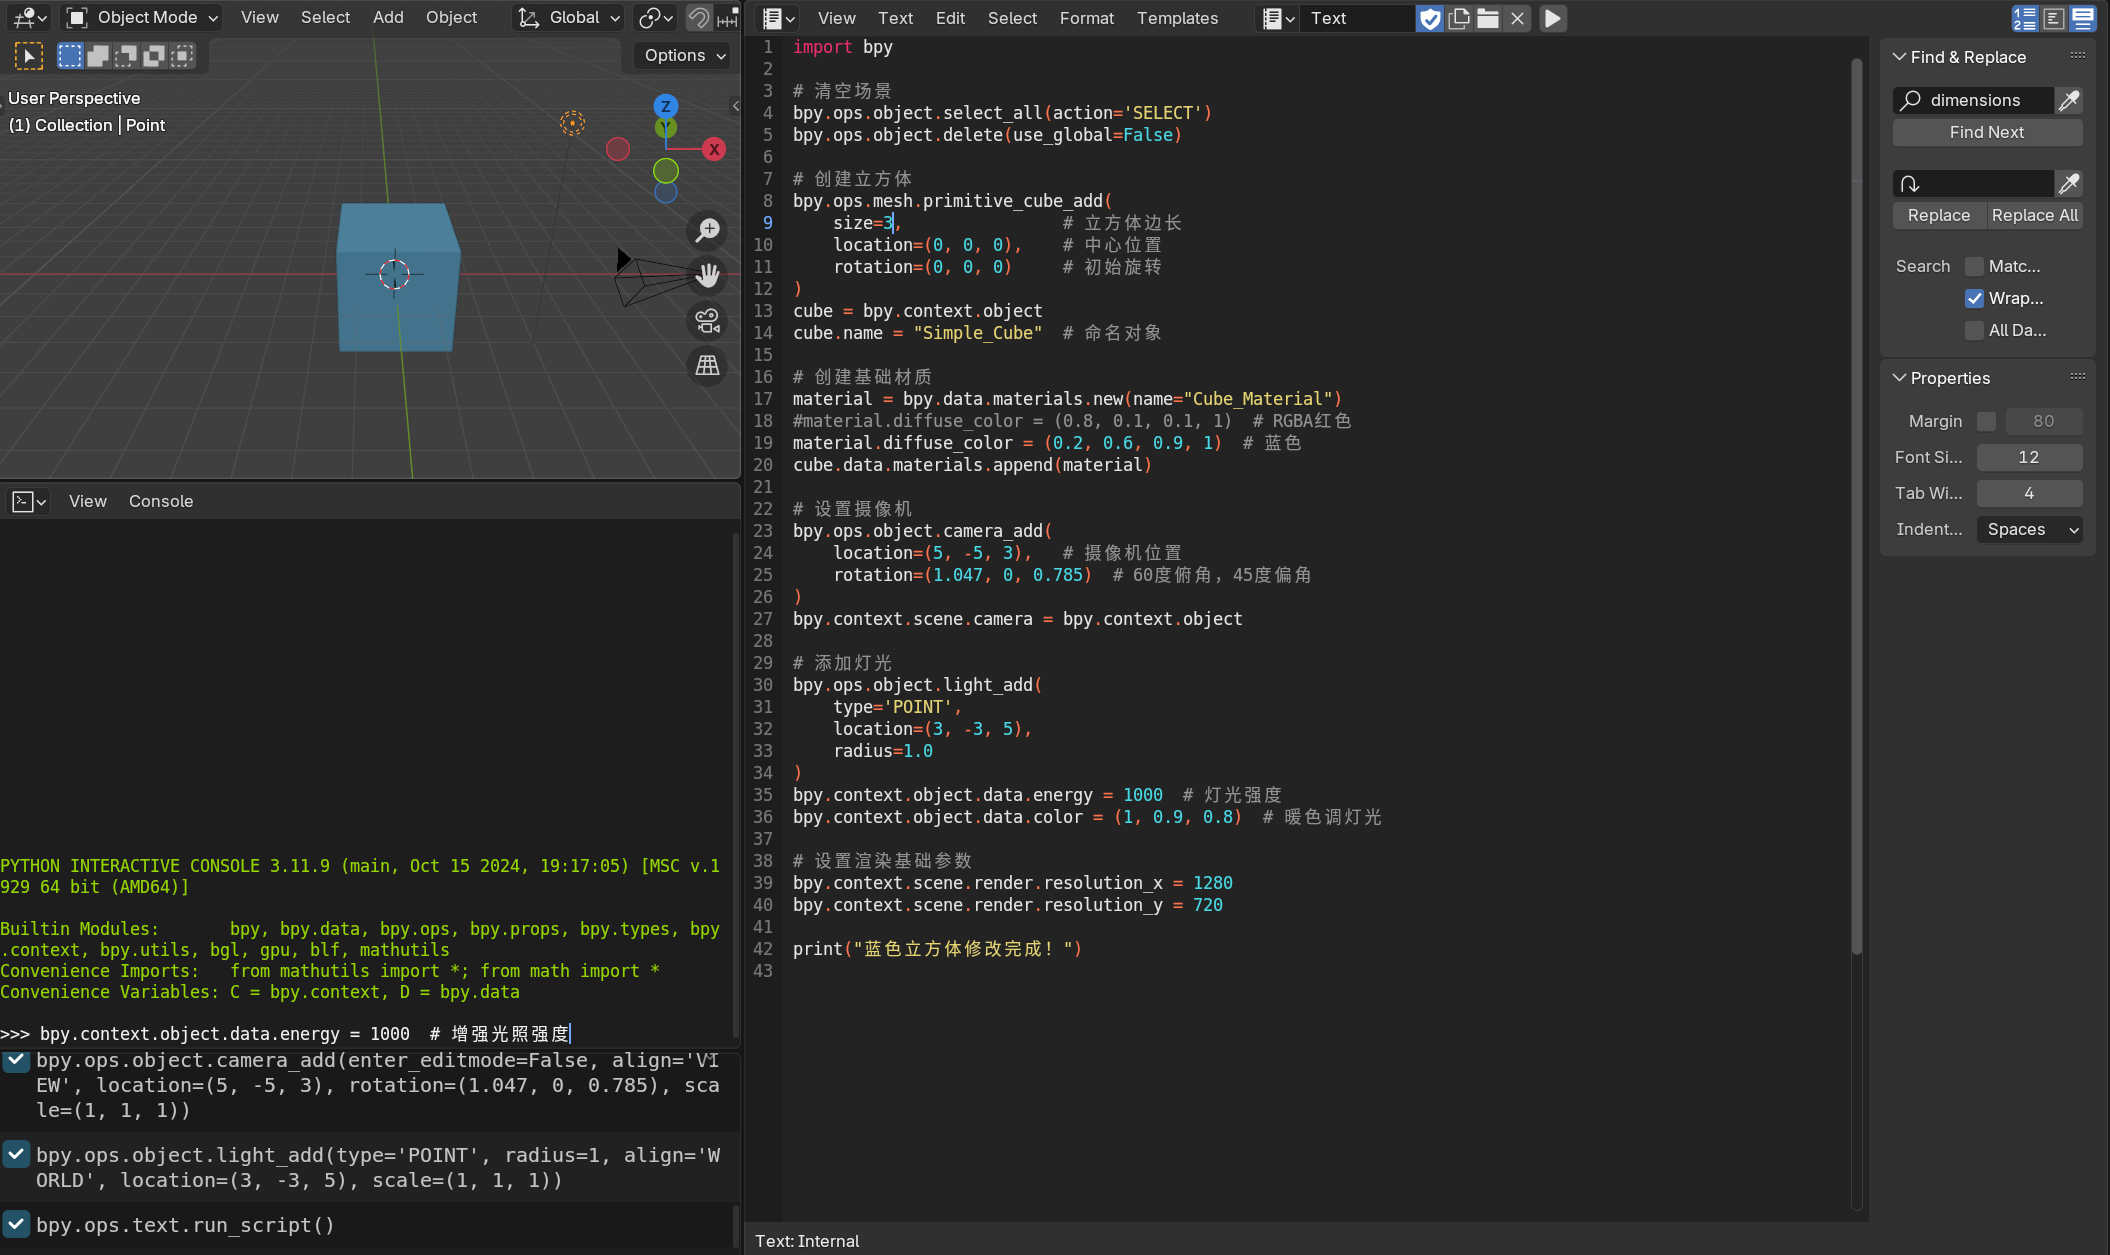
\includegraphics[width=0.7\textwidth]{assets/figures/修改后效果图.jpg} %插入图片,[]中设置图片大小,{}中是图片文件名
  \caption{修改后效果图} %最终文档中希望显示的图片标题
  \label{fig:3d-red-cube-changed} %用于文内引用的标签
}

\subsection{动手试试看}
AI提示词示例 
改变物体形状:
\prompt{将立方体改为球体}\\
调整场景光照:
\prompt{添加三点照明系统} \\
制作简单动画:
\prompt{创建旋转动画效果} \\
% \section{GPT辅助开发与代码编写}\label{sec:gpt-code}


在这个数字化时代,编程已经成为连接人类智慧与机器世界的桥梁。从智能手机到人工智能,每一行代码都在构建着我们未来的数字文明。但编程并非易事,它需要深奥的知识、严谨的逻辑和丰富的经验。

而GPT(生成式预训练变换模型)的出现,正在改变这一现状。这项革命性的技术不仅能够理解人类的语言,更能理解和生成高质量的代码。这不仅是技术创新的进步,更是人类智慧与机器智能融合的新起点。

本节将带读者进入这个激动人心的技术领域,探索GPT如何成为每一位开发者的强大助力。无论您是编程新手还是经验丰富的开发者,都将在这里发现新的可能性,开启代码创作的新纪元。

\subsection{使用GPT进行代码开发}\label{sec:gpt-dev}

在传统的软件开发过程中,开发者面临着一系列复杂且相互关联的任务。首先,需求理解是软件开发的起点,开发者需要将业务需求准确地转化为技术实现的方案。这一过程不仅要求开发者具备对业务的深刻洞察力,还需要他们能够将非技术性的需求转化为清晰、可操作的技术目标。随后,系统设计阶段要求开发者规划整个系统的架构和模块划分,这需要他们在宏观层面把握系统的整体结构,同时确保各个模块之间的协同性和可扩展性。编码实现阶段则是将设计转化为实际代码的过程,开发者需要编写高质量的代码,以确保软件的性能和可靠性。最后,测试与维护阶段是软件开发的收尾环节,开发者需要确保代码的稳定性和可维护性,以便在软件的生命周期中持续优化和更新。这些环节不仅耗时耗力,还要求开发者具备跨领域的知识,涉及业务理解、架构设计、编程技能以及质量保证等多个方面。

然而,随着人工智能技术的飞速发展,特别是像 GPT 这样的大型语言模型的出现,为解决这些传统软件开发中的难题提供了新的思路和方法。这些模型能够通过自然语言理解与生成的能力,辅助开发者在需求理解阶段更准确地把握业务需求,甚至自动生成初步的设计方案和代码框架。在测试与维护阶段,它们也能提供自动化测试脚本生成和代码优化建议等支持,从而显著提高软件开发的效率和质量。

GPT 作为一种先进的人工智能语言模型,正在通过多种方式深刻地改变传统的软件开发模式。首先,它能够实现自动化生成文档的功能,这使得开发者可以高效地根据现有代码自动生成 API 说明和用户手册等文档资料。这种自动化文档生成不仅节省了开发者在文档编写上的大量时间,还确保了文档与代码的一致性和准确性,从而提高了开发效率和软件交付的质量。
其次,GPT 在智能代码审查方面发挥着重要作用。它能够对代码进行深度分析,提供有价值的改进意见,并帮助开发者发现潜在的问题。这种智能审查功能类似于一个虚拟的代码导师,能够在开发过程中及时指出代码中的不足之处,从而帮助开发者优化代码质量,减少错误和漏洞。
此外,GPT 还支持快速原型开发。开发者只需提供需求描述,GPT 就能够快速生成初始的代码框架。这种能力极大地缩短了从需求分析到代码实现的时间,使得开发者能够更快速地验证想法并进行迭代开发。快速原型开发不仅提高了开发效率,还降低了项目初期的风险,使团队能够更快地响应市场变化。
最后,GPT 提供了跨语言支持功能,能够在不同编程语言之间进行代码转换和适配。这一功能对于多语言开发环境尤为重要,它使得开发者能够在不同语言之间无缝切换,减少了因语言差异带来的开发障碍。跨语言支持不仅提高了开发的灵活性,还促进了不同技术栈之间的协作和整合。

因此,选择 GPT 是因为它能够显著提高开发效率,减少重复性工作并加速流程;通过智能检查提升代码质量,增强稳定性和可维护性;有效连接业务需求与技术实现,弥合二者之间的鸿沟;同时为创新提供可能,探索传统方法难以触及的解决方案,从而推动软件开发向更高层次的效率、质量和创新能力迈进。这些功能不仅提高了开发效率,还提升了软件的整体质量,为软件开发领域带来了新的可能性和机遇。

下面通过实际的例子来展示GPT在开发中的应用。以网站开发为例,先介绍生成API文档,由用户输入代码片段,由GPT输出详细的接口说明:

\begin{promptbox}
\small{
\begin{lstlisting}[language=Python]
    // 用户输入一段REST API的代码
    GET /users
    Response:
    {
        "users": [
            {"id": 1, "name": "Alice"},
            {"id": 2, "name": "Bob"}
        ]
    }
\end{lstlisting}}
\end{promptbox}

\begin{gptbox}
\small{
\begin{lstlisting}[language=Python]
    // GPT生成的API文档
    ### 用户管理接口
    
    #### 获取用户列表
    ```http
    GET /api/users
    
    
    #### 响应格式
    {
        "users": [
            {"id": number, "name": string}
        ]
    }

    #### 错误码
    401: 未认证
    500: 内部错误
    ...
\end{lstlisting}
}
\end{gptbox}


除此之外,对于已经编写好的代码,用户还可以使用GPT对代码审查与优化,用户原始代码输入如下:

\begin{promptbox}
\small{\begin{lstlisting}[language=Python]
    # 用户输入的原始代码
    def calculate_average(numbers):
        sum = 0
        for number in numbers:
            sum += number
        average = sum / len(numbers)
        return average
\end{lstlisting}}
\end{promptbox}

\begin{gptbox}
\small{
\begin{lstlisting}[language=Python]
    # GPT建议的优化版本
    def calculate_average(numbers):
        """计算数字列表的平均值"""
        if not numbers:
            return 0.0
        return sum(numbers) / len(numbers)
\end{lstlisting}
}
\end{gptbox}

快速原型开发是GPT在代码开发的重要应用,体现了GPT独立完成开发项目的能力。从用户需开始,描述如下:

\prompt{需要一个在线投票系统,用户可以创建投票、查看结果统计。}


\begin{gptbox}
\small{
\begin{lstlisting}[language=Python]
    # models.py
    class Poll(models.Model):
        title = models.CharField(max_length=200)
        description = models.TextField()
        created_at = models.DateTimeField(auto_now_add=True)
        votes = models.ManyToManyField(User, through='Vote')
    
    class Vote(models.Model):
        user = models.ForeignKey(User, on_delete=models.CASCADE)
        poll = models.ForeignKey(Poll, on_delete=models.CASCADE)
        choice = models.CharField(max_length=200)
    
    # views.py
    @login_required
    def create_poll(request):
        if request.method == 'POST':
            form = PollForm(request.POST)
            if form.is_valid():
                poll = form.save(commit=False)
                poll.created_by = request.user
                poll.save()
                return redirect('poll_list')
        else:
            form = PollForm()
        return render(request, 'create_poll.html', {'form': form})
\end{lstlisting}
}
\end{gptbox}


\subsection{使用GPT进行代码编写}

在日常编程实践中,开发者常常遭遇诸多棘手难题,这些问题不仅影响开发效率,还可能引发潜在的软件质量问题。首先,语法错误是编程中常见的问题,包括拼写错误、括号不匹配等,这些问题虽小,却能导致程序无法正常编译或运行。其次,逻辑问题往往更具挑战性,例如算法的实现、复杂的条件判断以及程序流程的控制,这些问题需要开发者具备深入的逻辑思维能力和丰富的编程经验。此外,代码风格的统一性也是一个不容忽视的问题,保持代码的一致性和可读性对于团队协作和后续维护至关重要,然而在实际开发中,由于不同开发者编程习惯的差异,代码风格往往难以统一。最后,知识获取也是开发者面临的一大挑战,快速准确地查找 API、框架的使用方法以及相关技术文档,对于高效开发至关重要,但在海量信息中筛选出准确、有用的内容并非易事。

在这种背景下,GPT 的出现为解决上述问题提供了创新性的思路和方法。凭借其强大的语义理解和生成能力,GPT 能够在多个层面为开发者提供支持。它不仅可以帮助开发者快速识别和纠正语法错误,还能通过逻辑分析和代码优化建议,协助解决复杂的逻辑问题。此外,GPT 还能够提供代码风格指南和格式化建议,帮助开发者保持代码的一致性和可读性。更重要的是,GPT 能够快速响应开发者关于 API 和框架使用方法的查询,提供准确的技术信息,从而显著提升开发效率并降低知识获取的门槛。

同时,在软件开发领域,编码效率的提升是开发者不懈追求的目标。GPT 作为一种先进的人工智能工具,为这一目标的实现提供了强有力的支持。首先,GPT 的智能代码补全功能能够根据上下文环境精准预测下一步代码,极大地减少了开发者手动输入代码的时间,同时降低了因拼写错误或语法不规范而导致的编译问题。其次,GPT 能够识别代码中的错误,并提供针对性的修正建议,这不仅帮助开发者快速定位问题,还提升了代码的可靠性和稳定性。此外,GPT 还具备代码风格调整的能力,能够统一代码格式并优化变量命名,从而增强代码的可读性和一致性。最后,GPT 可以即时获取 API 说明和使用示例,为开发者提供技术文档查找的便捷途径,显著减少了在海量信息中搜索所需知识的时间成本。

选择 GPT 作为开发辅助工具,不仅因其能够提供即时帮助,随时为开发者提供编程指导和建议,还在于其能够显著提升代码质量。通过智能纠错功能,GPT 有效减少了潜在的错误,增强了代码的可靠性,从而为软件的稳定性和可维护性奠定了坚实基础。此外,GPT 的使用大幅节省了开发者查找资料的时间成本,使他们能够将更多精力集中在核心逻辑的实现上。更为重要的是,GPT 能够启发开发者探索新的解决方案和实现方式,为软件开发带来创新思路。这些优势共同构成了 GPT 在软件开发领域广泛应用的重要原因,使其成为开发者提升编码效率和质量的得力助手。

为了充分发挥GPT的代码编写能力,下面演示根据自然语言生成代码的过程。

\prompt{我需要一个函数,可以计算两个数的和,并返回结果。}

\begin{gptbox}
\footnotesize{使用如下代码可以实现上述功能:}
\small{
\begin{lstlisting}[language=Python]
    def add_numbers(a, b):
        """Calculate the sum of two numbers."""
        return a + b
\end{lstlisting}
}
\end{gptbox}

\prompt{print("Hello World!)这行代码有没有错误?}

\begin{gptbox}
\footnotesize{检测到缺少引号,应修正为:}
\small{
\begin{lstlisting}[language=Python]
    print("Hello World!")
\end{lstlisting}
}
\end{gptbox}


\begin{promptbox}
\footnotesize{下面的代码效率如何,能不能改进?}
\small{
\begin{lstlisting}[language=Python]
    total = 0
    for num in numbers:
        total += num
    average = total / len(numbers)
\end{lstlisting}}
\end{promptbox}

\begin{gptbox}
\footnotesize{可以使用更简洁的方式:}
\small{
\begin{lstlisting}[language=Python]
    average = sum(numbers) / len(numbers) if numbers else 0
\end{lstlisting}
}
\end{gptbox}



\begin{promptbox}
\footnotesize{帮我统一命名规范}
\small{
\begin{lstlisting}[language=Python]
    function getUserName(id) {
        return users[id].name;
    }
    
    function GetUserEmail(id) {
        return users[id].email;
    }
\end{lstlisting}}
\end{promptbox}

\begin{gptbox}
\footnotesize{以下是统一后的结果}
\small{
\begin{lstlisting}[language=Python]
    function getUserInfo(id, field) {
        return users[id][field];
    }
\end{lstlisting}
}
\end{gptbox}

\subsection{动手试试:明文加密}

正所谓古人云:``学而不思则罔,思而不学则殆''。在前面的介绍中,已经有了实例演示的例子。那么现在我们再尝试动手使用GPT写几个小例子吧\textasciitilde{}。

\textbf{案例一:摩尔斯电码(Morse code)}也被称作摩斯密码,是一种时通时断的信号代码,通过不同的排列顺序来表达不同的英文字母、数字和标点符号。它发明于1837年,是一种早期的数字化通信形式。不同于现代化的数字通讯,摩尔斯电码只使用零和一两种状态的二进制代码,它的代码包括五种:短促的点信号``・'',保持一定时间的长信号``---'',表示点和划之间的停顿、每个词之间中等的停顿,以及句子之间长的停顿。
读者往往会在在众多影视作品中可以看到摩尔斯电码,那么现在我们就让GPT来完成一个这样的简单例子。

\prompt{现在我想编写一个将自然语言转化为摩斯密码的代码,使用Python代码实现,就以''I LIKE U``这个句子为例实现一下。}

\begin{gptbox}
\footnotesize{为了将自然语言句子转换为摩斯密码,我们可以按照以下步骤实现:

\begin{enumerate}
  \def\labelenumi{\arabic{enumi}.}
  \item
        \textbf{创建摩斯密码字典}:包含所有英文字母及其对应的摩斯码。
  \item
        \textbf{处理输入字符串}:将其转为大写,并去除非字母字符,分割成单词列表。
  \item
        \textbf{转换每个单词}:将每个字母转换为摩斯码,并用单个空格分隔。
  \item
        \textbf{合并单词间的摩斯码}:使用三个空格分隔不同单词。
\end{enumerate}
以下是完整的Python代码:
}
\small{
以下是统一后的结果:
\begin{lstlisting}[language=Python]
    # 创建摩斯密码字典
    mos_codes = {
        'A': '.-', 'B': '-...', 'C': '-.-.', 'D': '-..', 'E': '.', 
        'F': '..-.', 'G': '--.', 'H': '....', 'I': '..', 'J': '.---', 
        'K': '-.-', 'L': '.-..', 'M': '--', 'N': '-.', 'O': '---', 
        'P': '.--.', 'Q': '--.-', 'R': '.-.', 'S': '...', 'T': '-', 
        'U': '..-', 'V': '...-', 'W': '.--', 'X': '-..-', 'Y': '-.--', 
        'Z': '--..'
    }
    
    # 获取输入并处理
    input_str = input("请输入要转换的句子:").upper()
    cleaned = ''.join([c if c in mos_codes or c == ' ' else '' for c in input_str])
    words = cleaned.split()
    
    # 转换为摩斯码
    morse_words = []
    for word in words:
        morse_word = [mos_codes[char] for char in word]
        morse_words.append(' '.join(morse_word))
    
    # 合并单词之间的空格
    final_morse = '   '.join(morse_words)
    print(final_morse)
\end{lstlisting}
}
\end{gptbox}

这段代码能够将输入句子转换为对应的摩斯密码,每个字母用单个空格分隔,单词之间用三个空格分隔。
通过本地运行代码并输出字符串``I LIKE U'',读者将得到上面实例的最终输出结果``.. .-.. .. -.- . ..-'',如\reffig{fig:morse}所示。

\fig[h]{
    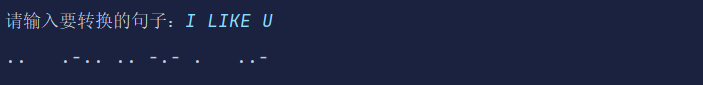
\includegraphics[width=0.7\textwidth]{assets/figures/image-20250210171257118.png} %插入图片,[]中设置图片大小,{}中是图片文件名
    \caption{摩斯密码输出} %最终文档中希望显示的图片标题
    \label{fig:morse} %用于文内引用的标签
}

现在读者可以用摩斯密码对你想说的文字进行加密了,读者还可以尝试继续让GPT改进,让这个简单代码不断完善并且可以处理中文相关的信息。

\textbf{案例二:恺撒密码(Caesar cipher)},或称\textbf{恺撒加密}、\textbf{恺撒变换}、\textbf{变换加密},是一种最简单且最广为人知的加密技术。它是一种替换加密的技术,明文中的所有字母都在字母表上向后(或向前)按照一个固定数目进行偏移后被替换成密文。例如,当偏移量是3的时候,所有的字母A将被替换成D,B变成E,以此类推。这个加密方法是以罗马共和时期恺撒的名字命名的,当年恺撒曾用此方法与其将军们进行联系。

这次我们再尝试一个古典密码学中的经典加密,根据苏维托尼乌斯于公元二世纪写的《恺撒传》中的记载,恺撒曾用此方法对重要的军事信息进行加密,它的原理非常简单,就是将所有字母偏移固定的长度,如\reffig{fig:caesar}:

\fig[h]{
    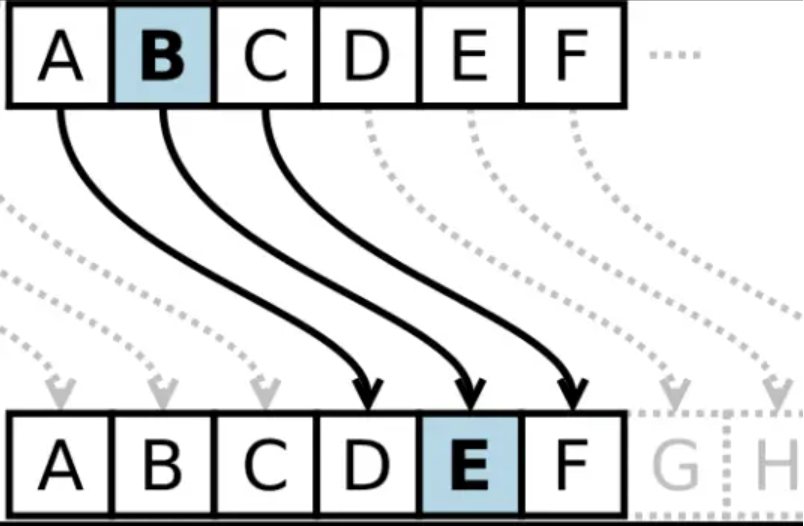
\includegraphics[width=0.5\textwidth]{assets/figures/image-20250210174403824.png} %插入图片,[]中设置图片大小,{}中是图片文件名
    \caption{恺撒加密示意图} %最终文档中希望显示的图片标题
    \label{fig:caesar} %用于文内引用的标签
}

那么现在我们同样用GPT来实现一个这样简单的例子:

\prompt{现在我想编写一个将自然语言转化为恺撒密码的代码,偏移量为3,使用Python代码实现,就以\texttt{My\ Fault\ forgive\ me\ for\ saying\ I\ like\ you\ here}这个句子为例实现一下。
}


\begin{gptbox}
\footnotesize{好的!凯撒密码是一种替换加密技术,每个字母在字母表上向后移动固定的位数(这里是3位)。例如,`A'会被转换为'D',`B'会变成'E',依此类推。对于字母表的末尾字母(如'X'、`Y'、`Z'),它们会循环回到字母表的开头。

以下是将自然语言转化为凯撒密码的Python代码实现:
}
\small{
\begin{lstlisting}[language=Python]
    def caesar_cipher(text, shift=3):
        result = []
        for c in text:
            if c.isupper():
                # 处理大写字母
                new_char = chr((ord(c) - ord('A') + shift) % 26 + ord('A'))
                result.append(new_char)
            elif c.islower():
                # 处理小写字母
                new_char = chr((ord(c) - ord('a') + shift) % 26 + ord('a'))
                result.append(new_char)
            else:
                # 非字母字符保持不变
                result.append(c)
        return ''.join(result)
    # 示例句子
    sentence = "My Fault forgive me for saying I like you here"
    encrypted_sentence = caesar_cipher(sentence, shift=3)
    print("加密后的句子:", encrypted_sentence)
\end{lstlisting}
}
\end{gptbox}

上述代码解释如下:

\begin{enumerate}
  \def\labelenumi{\arabic{enumi}.}

  \item
        \texttt{caesar\_cipher}函数接受两个参数:\texttt{text}(要加密的文本)和\texttt{shift}(偏移量,默认为3)。
  \item
        遍历输入文本中的每个字符。
  \item
        对于大写字母,计算其在字母表中的新位置,并将结果转换回字符。
  \item
        对于小写字母,同样进行处理。
  \item
        非字母字符(如空格、标点符号等)保持不变。
  \item
        将所有处理后的字符拼接成最终的加密字符串。
\end{enumerate}

最后,通过本地运行代码可以得到最终加密结果。输入句子:``My Fault forgive me for saying I like you here'',加密后的输出为``Pb Idxow irujlyh ph iru vdblqj L olnh brx khuh'',如\reffig{fig:caesar-example}。

\fig[h]{
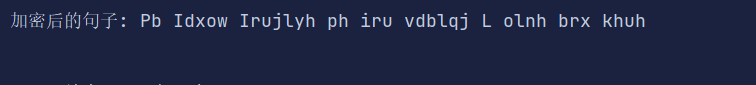
\includegraphics[width=0.7\textwidth]{assets/figures/image-20250210173814654.png} %插入图片,[]中设置图片大小,{}中是图片文件名
  \caption{恺撒加密输出图} %最终文档中希望显示的图片标题
  \label{fig:caesar-example} %用于文内引用的标签
}

Eulooldqw!(Brilliant!)现在你可以用恺撒密码对你想说的话进行加密了,你可以尝试继续让GPT改进,让它可以解密恺撒密码,动手试试看吧!

% \section{小结}

在当今数字化时代,人工智能生成内容(AIGC)正以前所未有的速度改变着我们的工作和学习方式。本章通过展示AIGC在文本、图像、音频和视频等多种形式内容生成中的应用,揭示了其强大的创造力和实用性。AIGC不仅能够快速生成高质量的内容,还能根据用户需求进行个性化定制,极大地提高了工作效率和学习效果。例如,通过自然语言处理技术,AIGC可以生成流畅且富有逻辑的文本,帮助用户快速撰写报告、文章或创意文案;在视觉艺术领域,它能够根据简单的描述生成精美的图像和设计,为设计师提供灵感;在音频和视频创作中,AIGC可以生成背景音乐、语音旁白甚至完整的视频内容,为多媒体制作开辟了新的可能性。这些应用不仅为专业人士提供了强大的工具,也为普通用户降低了创作门槛,使其能够轻松参与到内容创作中。然而,AIGC的发展也带来了版权、伦理和真实性等挑战,需要我们在使用过程中谨慎对待。随着技术的不断进步,AIGC将继续拓展其应用边界,成为未来工作和学习中不可或缺的助手。最终,AIGC将以AI agent的形式融入我们的日常生活,如\reffig{fig:ai-agent}所示,成为我们高效工作和深度学习的得力伙伴。

\fig[h]{
    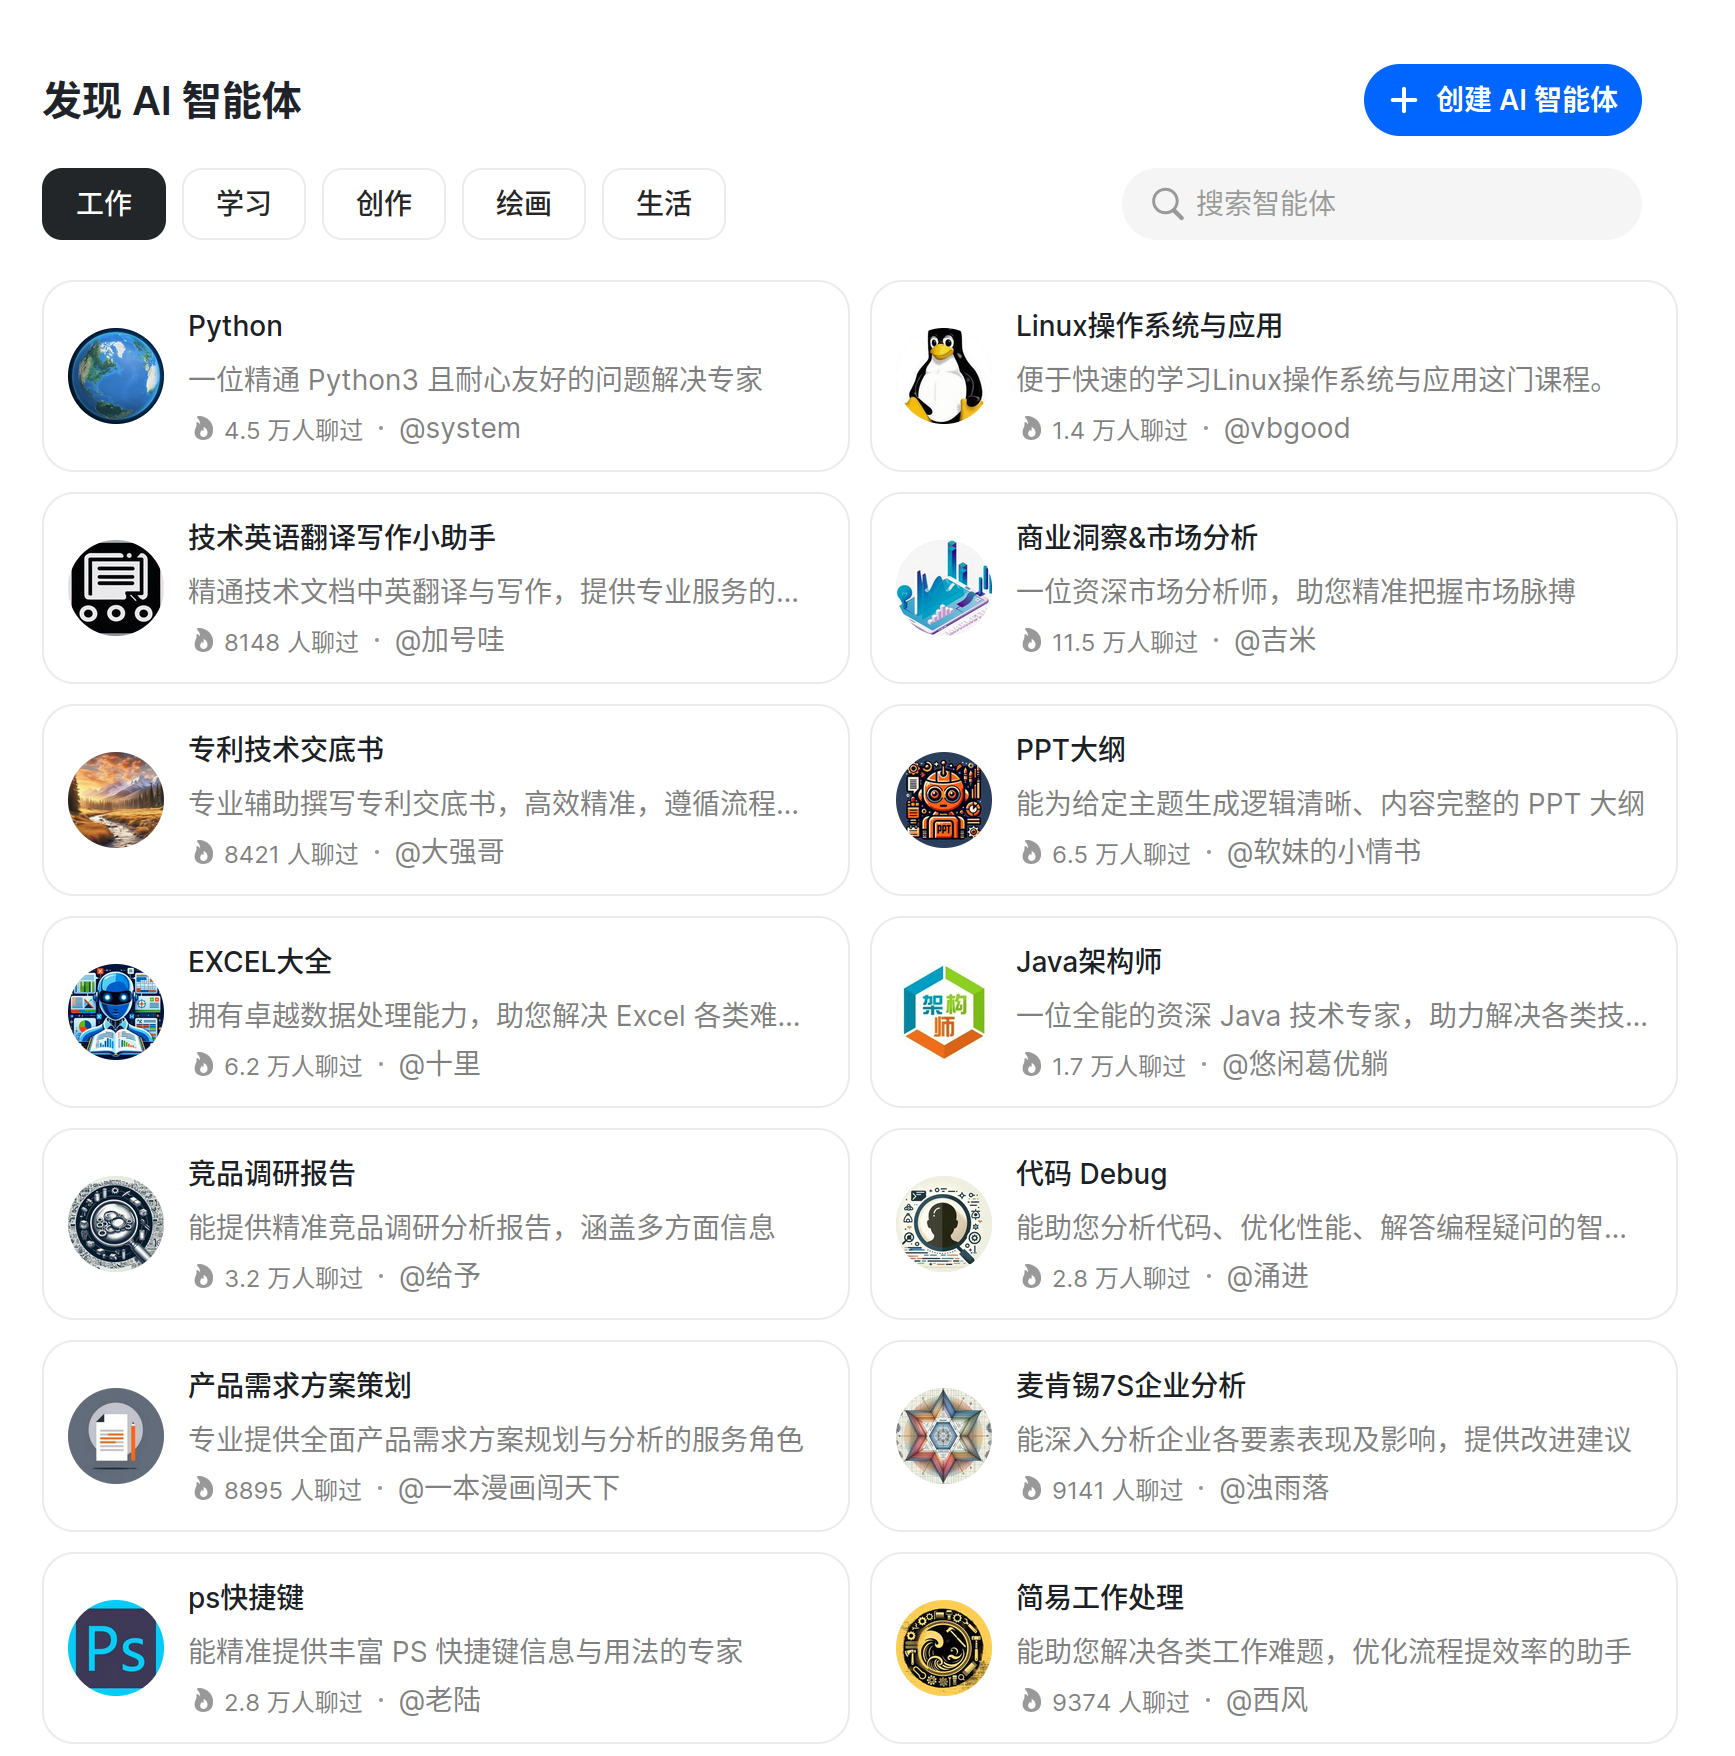
\includegraphics[width=0.7*\textwidth]{ai_agent}
    \caption{AI Agent}
    \label{fig:ai-agent}
}

% \bibliographystyle{plain}
% \bibliography{sections/d_references}
\end{document}